% Options for packages loaded elsewhere
\PassOptionsToPackage{unicode}{hyperref}
\PassOptionsToPackage{hyphens}{url}
%
\documentclass[
  english,
  man,floatsintext]{apa6}
\usepackage{amsmath,amssymb}
\usepackage{lmodern}
\usepackage{ifxetex,ifluatex}
\ifnum 0\ifxetex 1\fi\ifluatex 1\fi=0 % if pdftex
  \usepackage[T1]{fontenc}
  \usepackage[utf8]{inputenc}
  \usepackage{textcomp} % provide euro and other symbols
\else % if luatex or xetex
  \usepackage{unicode-math}
  \defaultfontfeatures{Scale=MatchLowercase}
  \defaultfontfeatures[\rmfamily]{Ligatures=TeX,Scale=1}
\fi
% Use upquote if available, for straight quotes in verbatim environments
\IfFileExists{upquote.sty}{\usepackage{upquote}}{}
\IfFileExists{microtype.sty}{% use microtype if available
  \usepackage[]{microtype}
  \UseMicrotypeSet[protrusion]{basicmath} % disable protrusion for tt fonts
}{}
\makeatletter
\@ifundefined{KOMAClassName}{% if non-KOMA class
  \IfFileExists{parskip.sty}{%
    \usepackage{parskip}
  }{% else
    \setlength{\parindent}{0pt}
    \setlength{\parskip}{6pt plus 2pt minus 1pt}}
}{% if KOMA class
  \KOMAoptions{parskip=half}}
\makeatother
\usepackage{xcolor}
\IfFileExists{xurl.sty}{\usepackage{xurl}}{} % add URL line breaks if available
\IfFileExists{bookmark.sty}{\usepackage{bookmark}}{\usepackage{hyperref}}
\hypersetup{
  pdftitle={How Do Like and Dislike Buttons Affect Communication? Testing the Privacy Calculus in a Preregistered One-Week Field Experiment},
  pdfauthor={Dienlin, Tobias1, Braeunlich, Katharina2, \& Trepte, Sabine3},
  pdflang={en-EN},
  pdfkeywords={privacy calculus, self-disclosure, popularity cues, field experiment, structural equation modeling, preregistration},
  hidelinks,
  pdfcreator={LaTeX via pandoc}}
\urlstyle{same} % disable monospaced font for URLs
\usepackage{graphicx}
\makeatletter
\def\maxwidth{\ifdim\Gin@nat@width>\linewidth\linewidth\else\Gin@nat@width\fi}
\def\maxheight{\ifdim\Gin@nat@height>\textheight\textheight\else\Gin@nat@height\fi}
\makeatother
% Scale images if necessary, so that they will not overflow the page
% margins by default, and it is still possible to overwrite the defaults
% using explicit options in \includegraphics[width, height, ...]{}
\setkeys{Gin}{width=\maxwidth,height=\maxheight,keepaspectratio}
% Set default figure placement to htbp
\makeatletter
\def\fps@figure{htbp}
\makeatother
\setlength{\emergencystretch}{3em} % prevent overfull lines
\providecommand{\tightlist}{%
  \setlength{\itemsep}{0pt}\setlength{\parskip}{0pt}}
\setcounter{secnumdepth}{-\maxdimen} % remove section numbering
% Make \paragraph and \subparagraph free-standing
\ifx\paragraph\undefined\else
  \let\oldparagraph\paragraph
  \renewcommand{\paragraph}[1]{\oldparagraph{#1}\mbox{}}
\fi
\ifx\subparagraph\undefined\else
  \let\oldsubparagraph\subparagraph
  \renewcommand{\subparagraph}[1]{\oldsubparagraph{#1}\mbox{}}
\fi
% Manuscript styling
\usepackage{upgreek}
\captionsetup{font=singlespacing,justification=justified}

% Table formatting
\usepackage{longtable}
\usepackage{lscape}
% \usepackage[counterclockwise]{rotating}   % Landscape page setup for large tables
\usepackage{multirow}		% Table styling
\usepackage{tabularx}		% Control Column width
\usepackage[flushleft]{threeparttable}	% Allows for three part tables with a specified notes section
\usepackage{threeparttablex}            % Lets threeparttable work with longtable

% Create new environments so endfloat can handle them
% \newenvironment{ltable}
%   {\begin{landscape}\begin{center}\begin{threeparttable}}
%   {\end{threeparttable}\end{center}\end{landscape}}
\newenvironment{lltable}{\begin{landscape}\begin{center}\begin{ThreePartTable}}{\end{ThreePartTable}\end{center}\end{landscape}}

% Enables adjusting longtable caption width to table width
% Solution found at http://golatex.de/longtable-mit-caption-so-breit-wie-die-tabelle-t15767.html
\makeatletter
\newcommand\LastLTentrywidth{1em}
\newlength\longtablewidth
\setlength{\longtablewidth}{1in}
\newcommand{\getlongtablewidth}{\begingroup \ifcsname LT@\roman{LT@tables}\endcsname \global\longtablewidth=0pt \renewcommand{\LT@entry}[2]{\global\advance\longtablewidth by ##2\relax\gdef\LastLTentrywidth{##2}}\@nameuse{LT@\roman{LT@tables}} \fi \endgroup}

% \setlength{\parindent}{0.5in}
% \setlength{\parskip}{0pt plus 0pt minus 0pt}

% \usepackage{etoolbox}
\makeatletter
\patchcmd{\HyOrg@maketitle}
  {\section{\normalfont\normalsize\abstractname}}
  {\section*{\normalfont\normalsize\abstractname}}
  {}{\typeout{Failed to patch abstract.}}
\patchcmd{\HyOrg@maketitle}
  {\section{\protect\normalfont{\@title}}}
  {\section*{\protect\normalfont{\@title}}}
  {}{\typeout{Failed to patch title.}}
\makeatother
\shorttitle{Popularity cues and privacy calculus}
\keywords{privacy calculus, self-disclosure, popularity cues, field experiment, structural equation modeling, preregistration\newline\indent Word count: 6073}
\usepackage{lineno}

\linenumbers
\usepackage{csquotes}
\setlength{\parskip}{0em}
\raggedbottom
\note{\clearpage}
\ifxetex
  % Load polyglossia as late as possible: uses bidi with RTL langages (e.g. Hebrew, Arabic)
  \usepackage{polyglossia}
  \setmainlanguage[]{english}
\else
  \usepackage[main=english]{babel}
% get rid of language-specific shorthands (see #6817):
\let\LanguageShortHands\languageshorthands
\def\languageshorthands#1{}
\fi
\ifluatex
  \usepackage{selnolig}  % disable illegal ligatures
\fi
\newlength{\cslhangindent}
\setlength{\cslhangindent}{1.5em}
\newlength{\csllabelwidth}
\setlength{\csllabelwidth}{3em}
\newenvironment{CSLReferences}[2] % #1 hanging-ident, #2 entry spacing
 {% don't indent paragraphs
  \setlength{\parindent}{0pt}
  % turn on hanging indent if param 1 is 1
  \ifodd #1 \everypar{\setlength{\hangindent}{\cslhangindent}}\ignorespaces\fi
  % set entry spacing
  \ifnum #2 > 0
  \setlength{\parskip}{#2\baselineskip}
  \fi
 }%
 {}
\usepackage{calc}
\newcommand{\CSLBlock}[1]{#1\hfill\break}
\newcommand{\CSLLeftMargin}[1]{\parbox[t]{\csllabelwidth}{#1}}
\newcommand{\CSLRightInline}[1]{\parbox[t]{\linewidth - \csllabelwidth}{#1}\break}
\newcommand{\CSLIndent}[1]{\hspace{\cslhangindent}#1}

\title{How Do Like and Dislike Buttons Affect Communication? Testing the Privacy Calculus in a Preregistered One-Week Field Experiment}
\author{Dienlin, Tobias\textsuperscript{1}, Braeunlich, Katharina\textsuperscript{2}, \& Trepte, Sabine\textsuperscript{3}}
\date{}


\note{

This preprint has been submitted to a journal and is currently under review. Please cite carefully.

}

\authornote{

Dr.~Tobias Dienlin is Assistant Professor of Interactive Communication at University of Vienna. He received his Ph.D.~from University of Hohenheim.

Dr.~Katharina Braeunlich works at the Federal Office for Information Security in Bonn. She is an alumna from University of Koblenz-Landau, where she received her Ph.D.

Dr.~Sabine Trepte is Full Professor for Media Psychology at University of Hohenheim. She received her Ph.D.~from Hanover University of Music, Drama and Media.

All authors contributed extensively to the work presented in this paper. TD, KB, \& ST designed the study; KB \& TD designed the online website; TD \& KB administered the data collection and importation; TD wrote the code, ran the models, and analyzed the output data; TD wrote the manuscript and ST provided comments; ST supervised the project.

The authors declare no competing interests.

This research was funded by the Volkswagen Foundation, project ``Transformations of privacy,'' which was awarded to Sandra Seubert, Sabine Trepte, Ruediger Grimm, \& Christoph Gusy. We would like to thank all our colleagues from the project as well as Niklas Johannes for valuable feedback.

This manuscript features a companion website, which includes the data, code, additional analyses, the preregistration, and a reproducible version of the manuscript (\url{https://XMtRa.github.io/privacy_calc_exp_anon}).

Correspondence concerning this article should be addressed to Dienlin, Tobias, University of Vienna, Department of Communication, 1090 Vienna, Austria. E-mail: \href{mailto:tobias.dienlin@univie.ac.at}{\nolinkurl{tobias.dienlin@univie.ac.at}}

}

\affiliation{\vspace{0.5cm}\textsuperscript{1} University of Vienna\\\textsuperscript{2} University of Koblenz-Landau\\\textsuperscript{3} University of Hohenheim}

\abstract{
According to privacy calculus, both privacy concerns and expected gratifications explain self-disclosure online. So far, most findings were based on self-reports or short-term experiments, and it is still largely unknown how popularity cues such as like and dislike buttons affect privacy calculus. To answer these questions we ran a preregistered one-week field experiment. Participants were randomly distributed to three different websites, on which they discussed a current political topic. The websites featured either (a) like buttons, (b) like and dislike buttons, or (c) no like or dislike buttons, and were otherwise identical. The final sample consisted of NOT AVAILABLE participants. Although the originally preregistered model was rejected, the results showed that a considerable share of actual self-disclosure could be explained by privacy concerns, gratifications, privacy deliberation, trust, and self-efficacy. The impact of the popularity cues on self-disclosure and privacy calculus was negligible.
}



\begin{document}
\maketitle

Understanding why people disclose personal information online is a critical question for society and research.
Originally, it was assumed that online self-disclosure is erratic and that it cannot be predicted by people's personal beliefs, concerns, or attitudes.
Most prominently, the privacy paradox stated that people self-disclose vast amounts of personal information online \emph{despite} having substantial concerns about their privacy (Barnes, 2006; Taddicken \& Jers, 2011).

Somewhat surprisingly, and despite its popularity in the media (New York Public Radio, 2018), the privacy paradox has garnered comparatively little empirical support.
A recent meta-analysis reported a correlation between privacy concerns and self-disclosure on SNS of \emph{r} = -.13 (Baruh, Secinti, \& Cemalcilar, 2017), which shows that privacy concerns are indeed related to self-disclosure online.

Hence, rather than further pursuing the privacy paradox, a large share of current day research builds on the so-called \emph{privacy-calculus} (Laufer \& Wolfe, 1977).
The privacy calculus states that self-disclosure online can be explained---at least partly---by means of expected risks \emph{and} expected benefits (Krasnova, Spiekermann, Koroleva, \& Hildebrand, 2010).
By operationalizing expected risks as privacy concerns, several studies have shown that experiencing privacy concerns is related to disclosing less information online, whereas expecting benefits is related to disclosing more information online (Heirman, Walrave, \& Ponnet, 2013; Koohikamali, French, \& Kim, 2019).

However, although the privacy calculus has gained momentum in academic research, several important questions remain unanswered.

First, current research on the privacy calculus is often criticized for not explicitly focusing on the deliberation process behind self-disclosure.
According to critics (e.g., Knijnenburg et al., 2017), showing that both concerns and gratifications correlate with self-disclosure is not sufficient evidence for an explicit weighing process.
In this study, we therefore explicitly focus on the privacy deliberation process.

Second, we approach the privacy calculus from a theoretical perspective of bounded rationality.
It is likely that other factors next to risks and benefits also determine behavior.
We therefore extend the privacy calculus model theoretically by investigating the role and interplay of trust and self-efficacy.

Third, the privacy calculus does not take place in a vacuum, and it is often argued that self-disclosure can be easily triggered by external circumstances.
We therefore analyze whether the privacy calculus is affected by the affordances of a website.
Specifically, we investigate whether \emph{popularity cues} such as like and dislike buttons affect the privacy calculus and whether they foster self-disclosure.

Fourth, it is still largely unknown whether the privacy calculus can be replicated with behavioral data in an authentic long-term setting (Kokolakis, 2017).
Thus far, most research on the privacy calculus used self-reports of behavior (Krasnova, Spiekermann, Koroleva, \& Hildebrand, 2010), vignette approaches (Bol et al., 2018), or one-shot experiments in the lab (Trepte, Scharkow, \& Dienlin, 2020).
A long-term field study in which actual behavior is observed in an authentic context is still missing.

To test our research questions, we collected a representative sample of the German population and conducted a preregistered online field experiment.
Participants were randomly distributed to one of three different websites, which either included a like button, both a like and a dislike button, or no buttons at all.
Over the course of one week participants had the chance to discuss a topical issue (i.e., prevention of terrorist attacks in Germany).
Afterward, they answered a follow-up questionnaire with items measuring the privacy calculus variables.

\hypertarget{the-privacy-calculus}{%
\subsection{The Privacy Calculus}\label{the-privacy-calculus}}

The key variable of interest for this study is self-disclosure.
Self-disclosure is a primary means of regulating privacy (e.g., Masur, 2018).
There are two different understandings of self-disclosure:
The first limits self-disclosure to \emph{deliberate} acts of sharing \emph{truthful} information about the self with others (Jourard, 1964).
The second considers \emph{all} acts of communication---active or passive, deliberate or unintended---as self-disclosure.
In other words, when communicating it is not possible not to self-disclose.
In this study, we adopt the latter understanding.
All types of communication allow for meaningful inferences about a person (Watzlawick, Bavelas, Jackson, \& O'Hanlon, 2011).
The recent years have illustrated vividly how much we can learn about a person only by analyzing their digital traces of communication or their meta-data (Kosinski, Stillwell, \& Graepel, 2013).
Self-disclosure has three different dimensions: breadth (i.e., number of topics covered), depth (i.e., intimacy of topics covered), and length (i.e., quantity of disclosure) (Omarzu, 2000).
Here, we focus on \emph{communication quantity}.
The more we communicate, the more we self-disclose.
Notably, the relation is not linear:
Impressions are formed quickly, and the more we communicate the less likely it becomes to share new information.

Privacy concerns were defined as follows:
``Concerns about online privacy represent how much an individual is motivated to focus on his or her control over a voluntary withdrawal from other people or societal institutions on the Internet, accompanied by an uneasy feeling that his or her privacy might be threatened'' (Dienlin, Masur, \& Trepte, 2019, p. 6).

In this study we adopt the theoretical perspective of the privacy calculus (Laufer \& Wolfe, 1977).
The privacy calculus assumes that when self-disclosing people engage in a rational weighing of risks and benefits.
We do not assume that this weighing process is flawless and that humans are perfect rational agents.
Instead, we understand the privacy calculus from the perspective of \emph{bounded rationality} (Simon, 1990).
Although humans weigh pros and cons when disclosing, their capacity is limited, errors happen, and manipulation always possible.

We therefore hypothesize that experiencing privacy concerns should reduce self-disclosure.
In light of bounded rationality and the existence of other competing factors that also influence self-disclosure, we assume that the effect is only small.
Previous research has likewise found that people who are more concerned about their privacy than others are slightly less likely to share personal information (Baruh, Secinti, \& Cemalcilar, 2017; Heirman, Walrave, \& Ponnet, 2013; Koohikamali, French, \& Kim, 2019).

H1: People are more likely to self-disclose on a website when they are less concerned about their privacy.

According to privacy calculus, the most relevant competing factor explaining self-disclosure is \emph{expected gratifications}.
People accept a loss of privacy if they can gain something in return (e.g., Laufer \& Wolfe, 1977).
The most prominent gratifications include social support (Krasnova, Spiekermann, Koroleva, \& Hildebrand, 2010), social capital (Ellison, Vitak, Steinfield, Gray, \& Lampe, 2011), entertainment (Dhir \& Tsai, 2017), information-seeking (Whiting \& Williams, 2013), and self-presentation (Min \& Kim, 2015).

H2: People are more likely to self-disclose on a website when they obtain more gratifications from using the website.

Privacy calculus holds that people deliberately compare benefits and disadvantages when disclosing.
However, that process has not been analyzed explicitly so far (Knijnenburg et al., 2017).
Only observing that privacy concerns and expected gratifications are related to self-disclosure is by itself not sufficient to prove an explicit weighing process.
Here, we suggest that the privacy calculus should be discussed in light of dual process theories, which state that people either deliberately, explicitly, and centrally take decisions, or instead do so automatically, implicitly, and peripherally (Kahneman, 2011; Petty \& Cacioppo, 1986).
Accordingly, privacy calculus would assume that people, when it comes to disclosing, engage in a central processing.
Building on Omarzu (2000) and Altman (1976), we hence introduce and investigate a novel concept termed \emph{privacy deliberation}.
Privacy deliberation captures the extent to which individual people explicitly compare potential positive and negative outcomes before communicating with others.

On the one hand, deliberating about privacy could \emph{reduce} subsequent self-disclosure.
Refraining from communication---the primary means of connecting with others---likely requires some active and deliberate restraint.
On the other hand, deliberating about privacy might also \emph{increase} self-disclosure.
A person concerned about their privacy might conclude that in this situation self-disclosure is actually beneficial.
Deliberation could represent some kind of inner consent, providing additional affirmation.
We therefore formulate the following research question:

RQ1: Are people more or less likely to self-disclose on a website depending on how actively they deliberate about whether they should self-disclose?

Bounded rationality implies that additional factors should also explain self-disclosure.
Self-disclosure online often takes place in situations where information is limited or obscure.
The more familiar users are with a context, the more experience, knowledge, and literacy they possess, the more likely they should be to navigate online contexts successfully.
In other words, if users possess more \emph{self-efficacy} regarding self-disclosing, they should also self-disclose more.
Related, people who report more privacy self-efficacy also engage in more self-withdrawal (Chen, 2018; Dienlin \& Metzger, 2016).

H3: People are more likely to self-disclose on a website when their self-efficacy about self-disclosing on the website is higher.

In situations where people lack experience or competence, the most relevant variable explaining behavior is, arguably, \emph{trust}.
Online, users often cannot control the context or the way their information is handled.
Trust therefore plays a key role in online communication (Metzger, 2004).
People who put more trust in the providers of networks, for example, disclose more personal information (Li, 2011).

Trust can be conceptualized in two different ways (Gefen, Karahanna, \& Straub, 2003).
It either captures ``\emph{specific} beliefs dealing primarily with the integrity, benevolence, and ability of another party'' (Gefen, Karahanna, \& Straub, 2003, p. 55, emphasis added).
Alternatively, it refers to a ``\emph{general} belief that another party can be trusted'' (Gefen, Karahanna, \& Straub, 2003, p. 55, emphasis added).
Whereas specific trust focuses on the causes of trust, general trust emphasizes the experience of trust.
In the online context, there exist several different \emph{targets} of trust, including (a) the information system, (b) the provider, (c) the Internet, and (d) the community of other users (Söllner, Hoffmann, \& Leimeister, 2016).

H4: People are more likely to self-disclose on a website when they have greater trust in the provider, the website, and the other users.

\hypertarget{the-effect-of-popularity-cues}{%
\subsection{The Effect of Popularity Cues}\label{the-effect-of-popularity-cues}}

So far we analyzed user-oriented factors that explain self-disclosure.
But how does the context, the digital infrastructure, affect the privacy calculus and self-disclosure?
In what follows we do not focus on specific \emph{features} of particular websites, which can change and quickly become obsolete (Fox \& McEwan, 2017).
Instead, we address the underlying latent structures by analyzing so-called \emph{affordances} (Ellison \& Vitak, 2015; Fox \& McEwan, 2017).
Developed by Gibson (2015), affordances emphasize that it is not the \emph{objective features} of objects that determine behavior, but our \emph{subjective perceptions}.
Affordances are mental representations of how objects might be used.

The privacy calculus states that both benefits and costs determine behavior.
Popularity cues such as like and dislike buttons, which are categorized as ``paralinguistic digital affordances'' (Carr, Hayes, \& Sumner, 2018, p. 142), can be linked tp the two sides of the privacy calculus.
The like button is positive and a potential benefit:
It expresses an endorsement, a compliment, a reward (Carr, Hayes, \& Sumner, 2018; Sumner, Ruge-Jones, \& Alcorn, 2017).
The dislike button is negative and a potential cost:
It expresses criticism and a way to downgrade content.

Paralinguistic digital affordances and specifically popularity cues can affect behavior (Krämer \& Schäwel, 2020; Trepte, Scharkow, \& Dienlin, 2020).
Online comments that already have several dislikes are much more likely to receive further dislikes (Muchnik, Aral, \& Taylor, 2013).
When users disagree with a post, they are more likely to click on a button labeled \emph{respect} compared to a button labeled \emph{like} (Stroud, Muddiman, \& Scacco, 2017).
In this vein, popularity cues likely also impact the privacy calculus (Krämer \& Schäwel, 2020).

Specifically, \emph{likes} are positive and represent the positivity bias typical of social media (Reinecke \& Trepte, 2014).
Receiving a like online is similar to receiving a compliment offline.
Introducing like-buttons mighty afford and emphasize a \emph{gain frame} (Rosoff, Cui, \& John, 2013).
These gains can be garnered only through participation.
Because like buttons emphasize positive outcomes, it is likely that concerns decrease.
In situations where there is more to win, people should also more actively deliberate about whether or not to disclose information.

H5. Compared to people who use a website without like or dislike buttons, people who use a website with like buttons (a) self-disclose more, (b) obtain more gratifications, (c) are less concerned about their privacy, and (d) deliberate more about whether they should communicate online.

Receiving a \emph{dislike} should feel more like a punishment.
Dislikes introduce a \emph{loss frame}.
As a result, websites featuring both like \emph{and} dislike buttons should be more ambivalent compared to websites without any popularity cues.
In online contexts, gains often outweigh losses.
Having both types of popularity cues might still lead to more gratifications and self-disclosure.
However, privacy concerns should not be reduced anymore:
People who are more concerned about their privacy are also more shy and risk averse (Dienlin, 2017).
Implementing the dislike button might therefore increase privacy concerns, thereby canceling out the positive effects of the like button.
And because there is more at stake, participants should deliberate even more whether or not to disclose.

H6. Compared to people who use a website without like or dislike buttons, people who use a website with like \emph{and} dislike buttons (a) self-disclose more, (b) obtain more gratifications, and (c) deliberate more about whether they should communicate online.

When directly comparing websites including both like and dislike buttons with websites including only like buttons, building on the rationales presented above, it is likely that websites including both buttons should increase privacy concerns and privacy deliberation.

H7. Compared to people who use a website with only like buttons, people who use a website with like and dislike buttons (a) are more concerned about their privacy, and (b) deliberate more about whether they should communicate online.

For a simplified overview of the model we analyzed, see Figure \ref{fig:model}.

\begin{figure}

{\centering 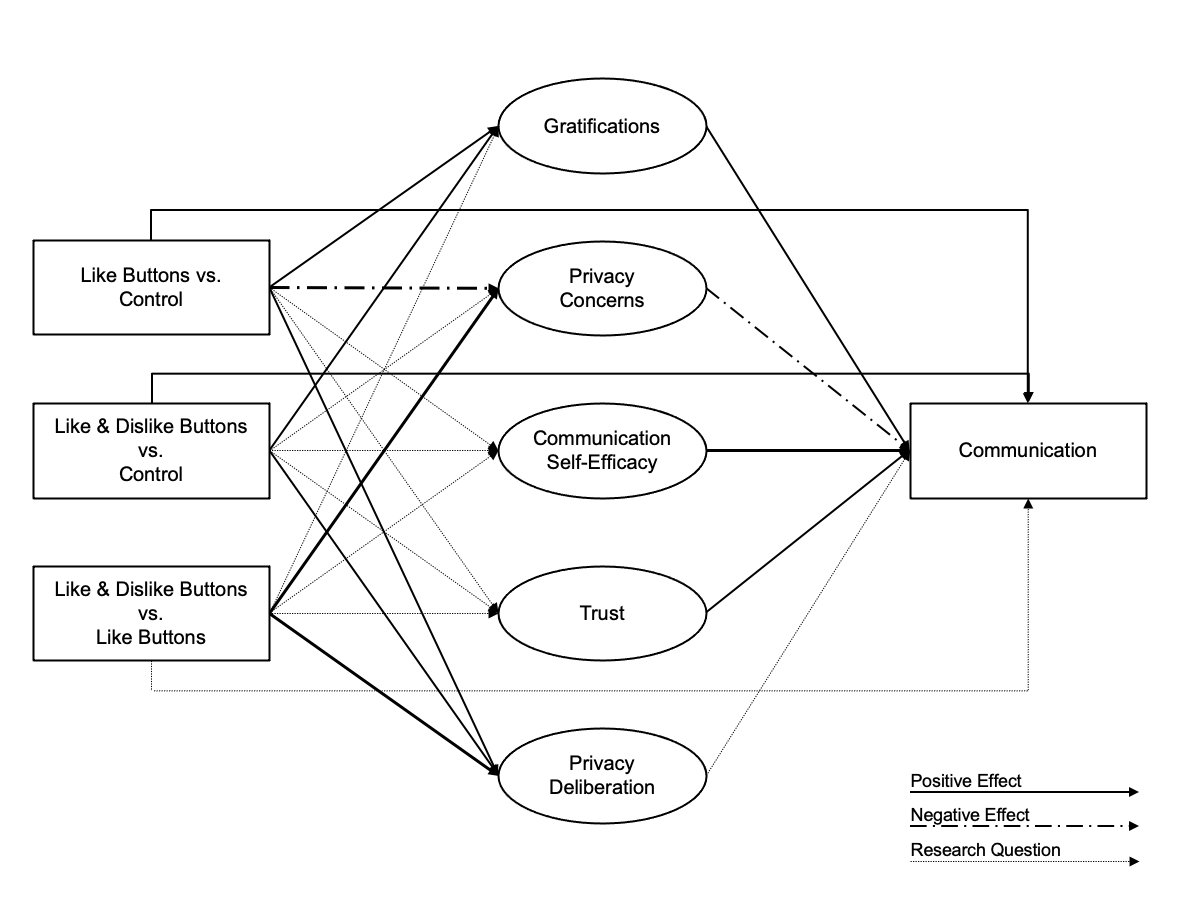
\includegraphics[width=.8\textwidth]{figures/design/model} 

}

\caption{Overview of analyzed model.}\label{fig:model}
\end{figure}

\hypertarget{methods}{%
\section{Methods}\label{methods}}

\hypertarget{open-science}{%
\subsection{Open Science}\label{open-science}}

The online supplementary material (OSM) of this study includes the data, research materials, analyses scripts, and a reproducible version of this manuscript, which can be found on the manuscript's companion website (\url{https://XMtRa.github.io/privacy_calc_exp_anon}).
We preregistered the study using the registration form \emph{OSF Prereg}, which includes the hypotheses, sample size, research materials, analyses, and exclusion criteria (see \url{https://osf.io/a6tzc/?view_only=5d0ef9fe5e1745878cd1b19273cdf859}).
We needed to change our pre-defined plan in some cases.
For a full account of all changes, see OSM.
New analyses that were not preregistered appear in the section Exploratory Analyses.

\hypertarget{procedure}{%
\subsection{Procedure}\label{procedure}}

The study was designed as an online field experiment with three different groups.
The first group used a website without like or dislike buttons, the second the same website but with only like buttons, and the third the same website but with both like and dislike buttons.
Participants were randomly distributed to one of the three websites in a between-subject design.

We collaborated with a market research company to recruit participants.
As incentive, participants were awarded digital points, which they could use to get special offers from other online commerce services.
Participants were above the age of 18 and lived in Germany.
In a first step, the company sent its panel members an invitation to participate in the study (\emph{invitation}).
In this invitation, panel members were asked to participate in a study analyzing the current threat posed by terrorist attacks in Germany.\footnote{Although the terror attack was not of primary interest for this study, the data can and will also be used to analyze perceptions of the terrorism threat. Hence, no deception took place, and in the debriefing participants were informed about our additional research interest in privacy.}
Members who decided to take part were subsequently sent the first questionnaire (\emph{T1}), in which we (a) asked about their sociodemographics, (b) provided more details about the study, and (c) included a registration link for the website, which was described as ``participation platform.''
Afterward, participants were randomly assigned to one of the three websites.
After registration was completed, participants were invited (but not obliged) to discuss the topic of the terrorism threat in Germany over the course of one week (\emph{field}).
Subsequently, participants received a follow-up questionnaire in which the self-reported measures were collected (\emph{T2}).
Measures were collected after and not before the field phase in order not to prime participants or reveal our primary research interest.

We programmed an online website based on the open-source software \emph{discourse} (\url{https://www.discourse.org/}).
We conducted several pretests with students from the local university to make sure the website had an authentic feel (see Figure \ref{fig:website}).
Participants used the website actively: Overall, they spent 162 hours online, wrote 1,171 comments, and clicked on 560 popularity cues.
Notably, we did not find any instances of people providing meaningless text.
For an example of communication that took place, see Figure \ref{fig:comments}.

\begin{figure}

{\centering 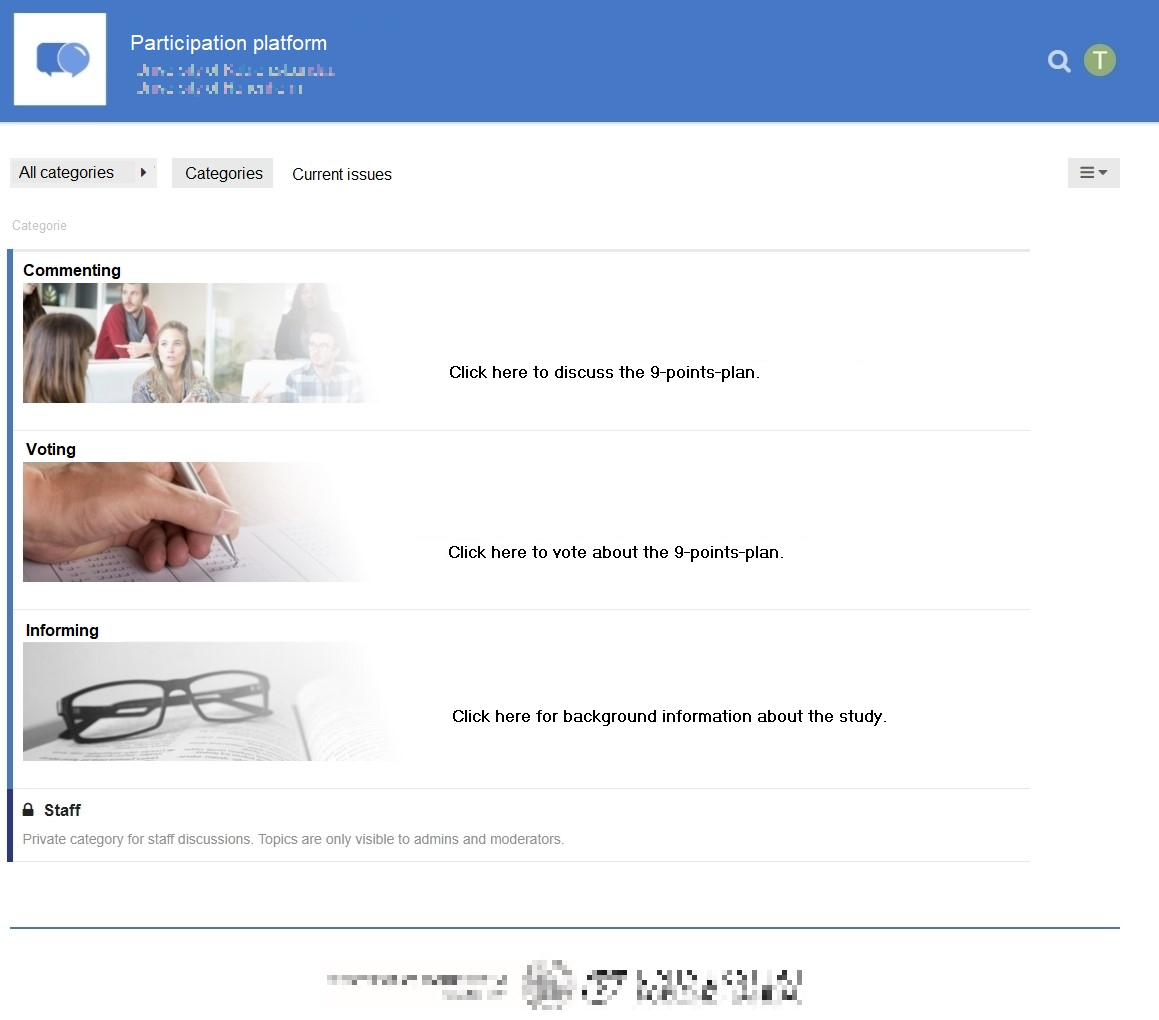
\includegraphics[width=.9\textwidth]{figures/website/website_translated} 

}

\caption{The website's homepage. (Translated to English.)}\label{fig:website}
\end{figure}

\begin{figure}

{\centering 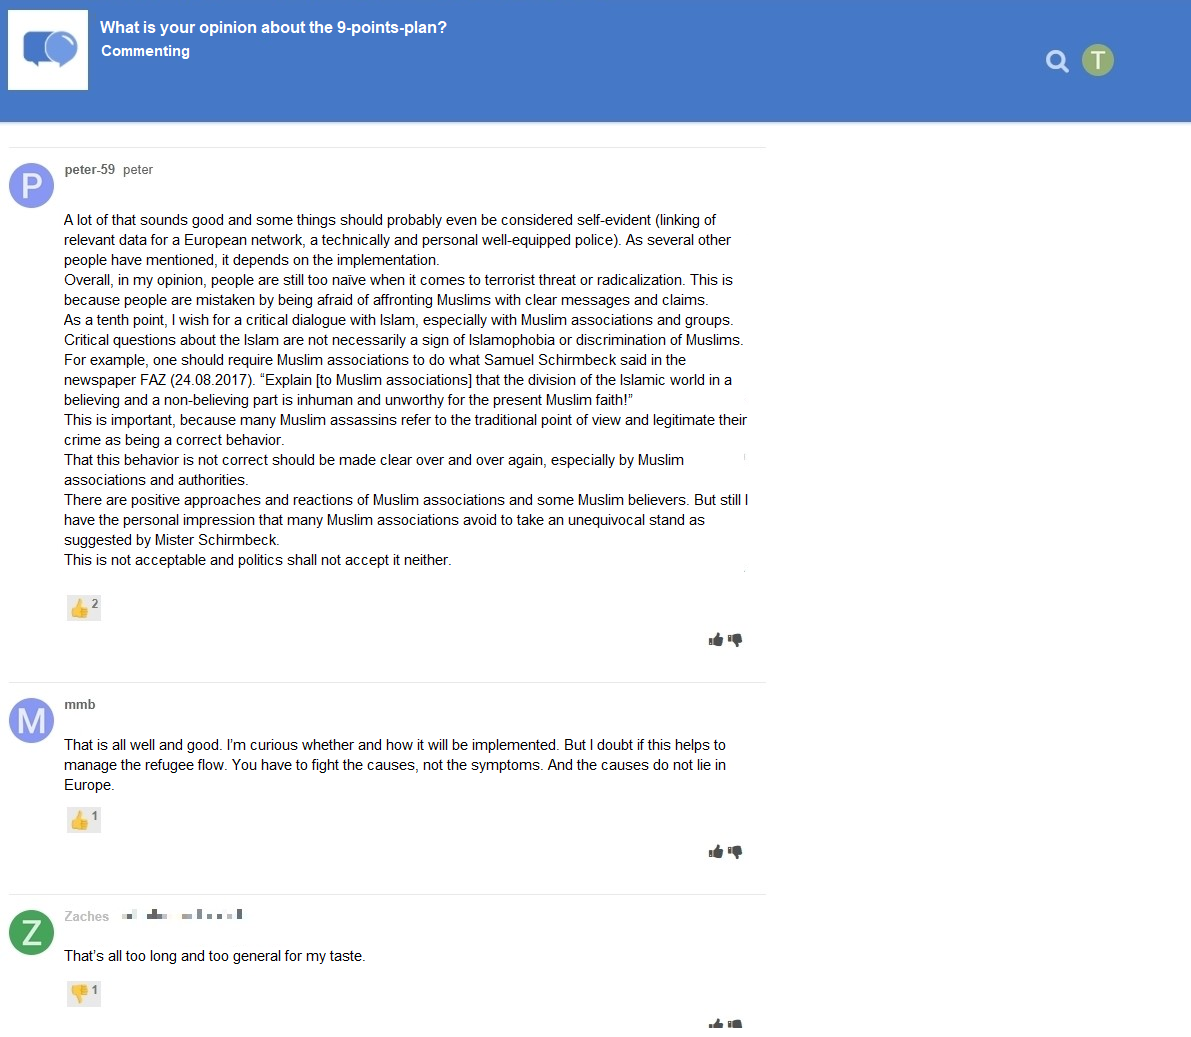
\includegraphics[width=.9\textwidth]{figures/website/comments_translated} 

}

\caption{Communication that took place on the website with like and dislike buttons. (Translated to English.)}\label{fig:comments}
\end{figure}

\hypertarget{participants}{%
\subsection{Participants}\label{participants}}

We ran a priori power analyses to determine sample size.
The power analysis was based on a smallest effect size of interest {[}SESOI; Lakens, Scheel, and Isager (2018){]}.
Namely, we defined a minimum effect size that we considered sufficiently large to support our hypotheses.
Because small effects should be expected when researching aspects of privacy online (e.g., Baruh, Secinti, \& Cemalcilar, 2017), with standardized small effects beginning at an effect size of \emph{r} = .10 (Cohen, 1992), we set our SESOI to be \emph{r} = .10.
Our aim was to be able to detect this SESOI with a probability of at least 95\%. Using the regular alpha level of 5\%, basic power analyses revealed a minimum sample size of \emph{N} = 1,077.
In the end, we were able to include \emph{N} = 559 in our analyses (see below).
This means that our study had a probability (power) of 77\% to find an effect at least as large as \emph{r} = .10.
Put differently, we were able to make reliable inferences (i.e., power = 95\%) about effects at least as big as \emph{r} = .14.

We collected a representative sample of the German population in terms of age, sex, and federal state.
In sum, 1,619 participants completed the survey at T1, 960 participants created a user account on the website, and 982 participants completed the survey at T2.
Using tokens and IP addresses, we connected the data from T1, participants' behavior on the website, and T2 by means of objective and automated processes.
The data of several participants could not be matched for technical reasons, for example because they used different devices for the respective steps.
In the end, the data of 590 participants could be matched successfully.
We excluded 29 participants who finished the questionnaire at T2 in less than three minutes, which we considered to be unreasonably fast.\footnote{We preregistered to delete participants with less than 6 minutes answer time. However, this led to the exclusion of too many data points of high quality, which is why we relaxed this criterion. In the OSM, we report also the results using all participants.}
To detect atypical data, we calculated Cook's distance.
We excluded two participants who provided clear response patterns (i.e., straight-lining).
The final sample included \emph{N} = 559 participants.
The sample characteristics at T1 and T2 were as follows:
T1: age = 45 years, sex = 49\% male, college degree = 22\%.
T2: age = 46 years, sex = 49\% male, college degree = 29\%.
One participant did not report their sex.

\hypertarget{measures}{%
\subsection{Measures}\label{measures}}

Wherever possible, we operationalized the variables using established measures.
Where impossible (for example, to date there exists no scale on privacy deliberation), we self-designed novel items, which were pretested concerning legibility and understandability.
To assess factor validity we ran confirmatory factor analyses (CFA).
If the CFAs revealed insufficient fit, we deleted malfunctioning items.
All items were formulated as statements to which participants indicated their (dis-)agreement on a bipolar 7-point scale.
Answer options were visualized as follows: -3 (\emph{strongly disagree}), -2 (\emph{disagree}), -1 (\emph{slightly disagree}), 0 (\emph{neutral}), +1 (\emph{slightly agree}), +2 (\emph{agree}), +3 (\emph{strongly agree}).
For the analyses, answers were coded from 1 to 7.
In the questionnaire, all items measuring a variable were presented on the same page in randomized order.

For an overview of the means, standard deviations, factorial validity, and reliability, see Table \ref{tab:CFA}.
For an overview of the variables' distributions, see Figure \ref{fig:corrplot}.
For the exact wording of all items and their individual distributions, see OSM.

\begin{table}[tbp]

\begin{center}
\begin{threeparttable}

\caption{\label{tab:CFA}Psychometric Properties, Factorial Validity, and Reliability of Measures}

\footnotesize{

\begin{tabular}{llllllllllll}
\toprule
 & \multicolumn{1}{c}{m} & \multicolumn{1}{c}{sd} & \multicolumn{1}{c}{chisq} & \multicolumn{1}{c}{df} & \multicolumn{1}{c}{pvalue} & \multicolumn{1}{c}{cfi} & \multicolumn{1}{c}{tli} & \multicolumn{1}{c}{rmsea} & \multicolumn{1}{c}{srmr} & \multicolumn{1}{c}{omega} & \multicolumn{1}{c}{ave}\\
\midrule
Privacy concerns & 3.21 & 1.51 & 11.04 & 9.00 & 0.27 & 1.00 & 1.00 & 0.02 & 0.01 & 0.96 & 0.80\\
General gratifications & 4.76 & 1.22 & 34.03 & 5.00 & 0.00 & 0.98 & 0.95 & 0.10 & 0.02 & 0.93 & 0.74\\
Specific gratifications & 4.71 & 1.02 & 269.77 & 85.00 & 0.00 & 0.94 & 0.93 & 0.06 & 0.05 & 0.95 & 0.59\\
Privacy deliberation & 3.93 & 1.29 & 15.55 & 5.00 & 0.01 & 0.98 & 0.96 & 0.06 & 0.02 & 0.85 & 0.53\\
Self-efficacy & 5.25 & 1.12 & 3.23 & 1.00 & 0.07 & 0.99 & 0.96 & 0.06 & 0.01 & 0.83 & 0.59\\
General trust & 5.21 & 1.04 & 2.07 & 1.00 & 0.15 & 1.00 & 0.99 & 0.04 & 0.01 & 0.87 & 0.70\\
Specific trust & 5.08 & 0.94 & 99.48 & 26.00 & 0.00 & 0.96 & 0.94 & 0.07 & 0.04 & 0.93 & 0.62\\
\bottomrule
\addlinespace
\end{tabular}

}

\begin{tablenotes}[para]
\normalsize{\textit{Note.} omega = Raykov's composite reliability coefficient omega; avevar = average variance extracted.}
\end{tablenotes}

\end{threeparttable}
\end{center}

\end{table}

\begin{figure}[!h]

{\centering 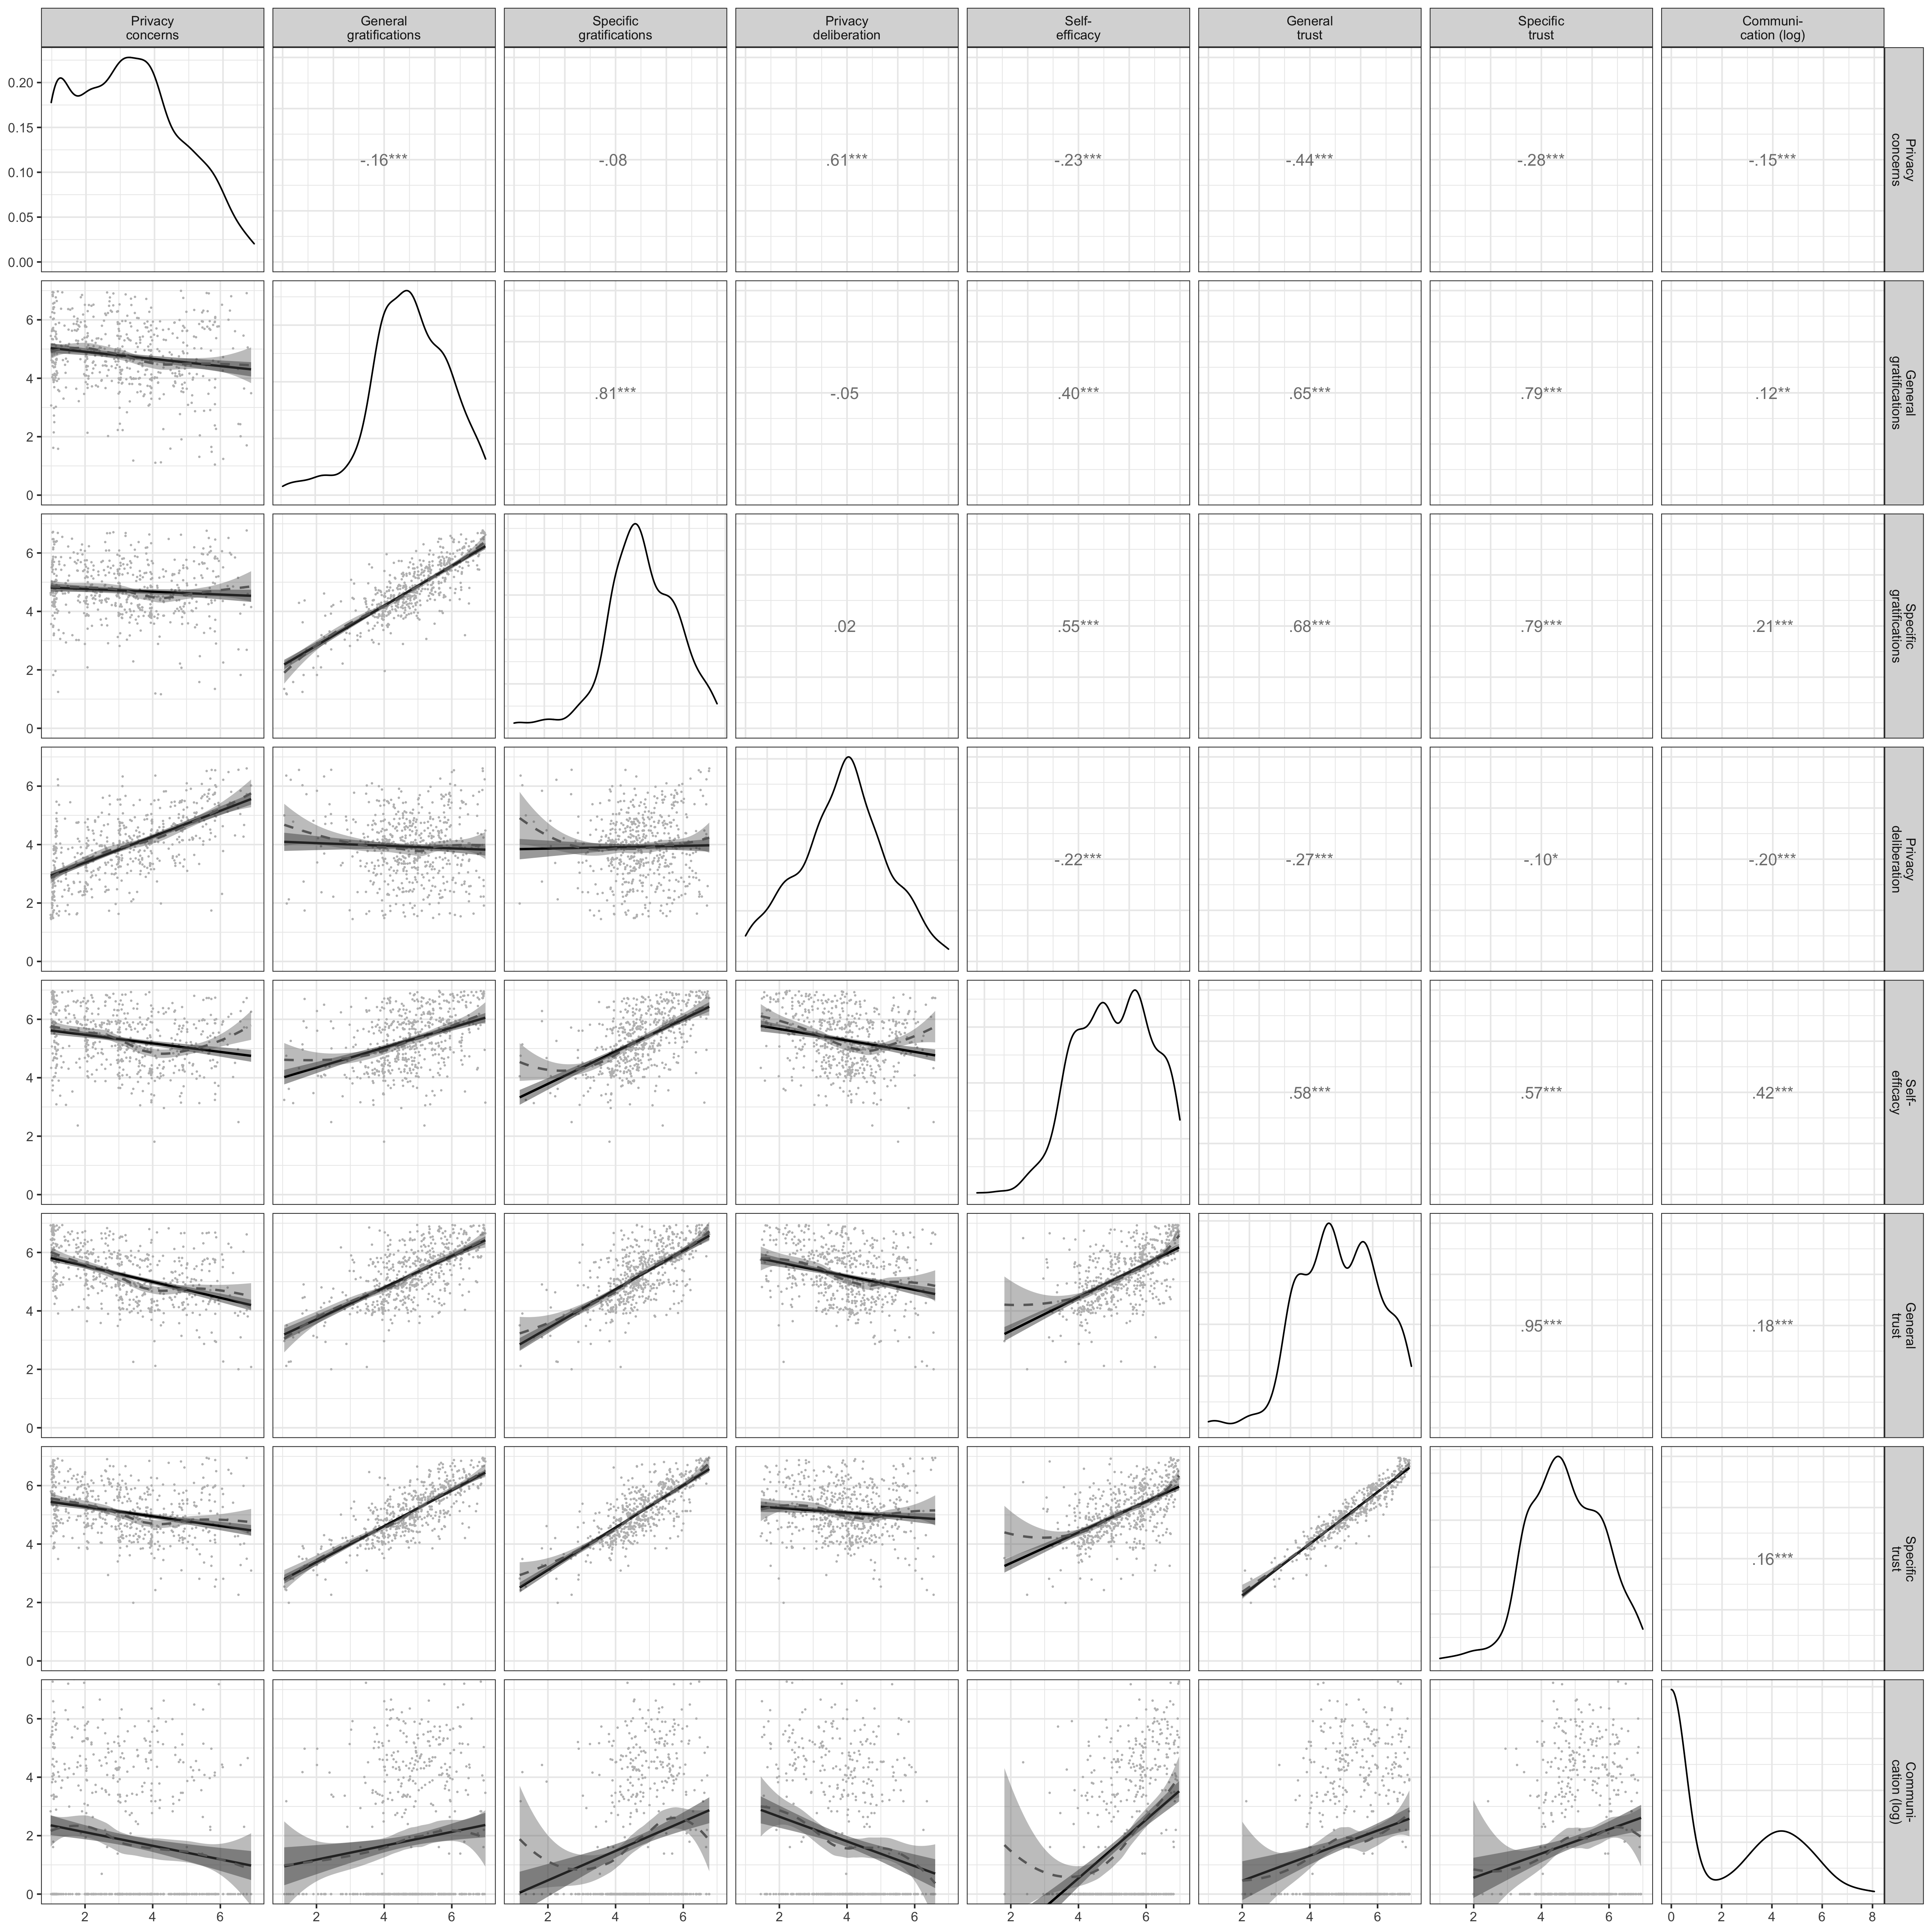
\includegraphics[width=.9\textwidth]{figures/results/cor_plot} 

}

\caption{Above diagonal: zero-order correlation matrix; diagonal: density plots for each variable; below diagonal: bivariate scatter plots for zero-order correlations. Solid regression lines represent linear regressions, dotted regression lines represent quadratic regressions. Calculated with the model predicted values for each variable (baseline model).}\label{fig:corrplot}
\end{figure}

\hypertarget{privacy-concerns}{%
\subsubsection{Privacy concerns}\label{privacy-concerns}}

Privacy concerns were measured with seven items based on Buchanan, Paine, Joinson, and Reips (2007).
One example item was ``When using the participation platform, I had concerns about my privacy.''
One item was deleted due to poor psychometric properties.

\hypertarget{gratifications}{%
\subsubsection{Gratifications}\label{gratifications}}

We differentiated between two separate types of gratifications.
\emph{General gratifications} were measured with five items based on Sun, Wang, Shen, and Zhang (2015).
One example item was ``Using the participation platform has paid off for me.''
\emph{Specific gratifications} were measured with 15 items on five different subdimensions with three items each.
The scale was based on Scherer and Schlütz (2002).
Example items were: ``Using the participation platform made it possible for me to'' \ldots{} ``learn things I would not have noticed otherwise'' (information), ``react to a subject that is important to me'' (relevance), ``engage politically'' (political participation), ``try to improve society'' (idealism), and ``soothe my guilty consciences'' (extrinsic benefits).

\hypertarget{privacy-deliberation}{%
\subsubsection{Privacy deliberation}\label{privacy-deliberation}}

Privacy deliberation was measured with five self-designed items. One example item was ``While using the participation platform I have weighed the advantages and disadvantages of writing a comment.''

\hypertarget{self-efficacy}{%
\subsubsection{Self-efficacy}\label{self-efficacy}}

Self-efficacy was captured with six self-designed items, which measured whether participants felt that they had sufficient self-efficacy to write a comment on the website.
For example, ``I felt technically competent enough to write a comment.''
Two inverted items were deleted due to poor psychometric properties.

\hypertarget{trust}{%
\subsubsection{Trust}\label{trust}}

We differentiated between two types of trust.
\emph{General trust} was operationalized based on Söllner, Hoffmann, and Leimeister (2016), addressing three targets (i.e., provider, website, and other users) with one item each.
One example item was ``The operators of the participation platform seemed trustworthy.''
\emph{Specific trust} was operationalized for the same three targets with three subdimensions each (i.e., ability, benevolence/integrity, and reliability), which were measured with one item each.
Example items were ``The operators of the participation platform have done a good job'' (ability), ``The other users had good intentions'' (benevolence/integrity), ``The website worked well'' (reliability).
The results showed that the provider and website targets were not sufficiently distinct, as was evidenced by a Heywood case (i.e., standardized coefficient greater than 1).
We hence adapted the scale to combine these two targets.
The updated scale showed adequate fit.

\hypertarget{self-disclosure}{%
\subsubsection{Self-disclosure}\label{self-disclosure}}

Self-disclosure was calculated by log-scaling of the number of words each participant wrote in a comment plus the double-weighted number of likes and dislikes (preregistered).
The number of likes and dislikes were multiplied by two because, rudimentarily, like buttons abbreviate the sentence ``I like'' and dislike buttons ``I dislike.''
The sum of words and likes/dislikes was log-scaled because the relative amount of self-disclosure decreases the more a person communicates (see above).

\hypertarget{data-analysis}{%
\subsection{Data analysis}\label{data-analysis}}

All hypotheses and research questions were tested using structural equation modeling with latent variables.
The influence of the three websites was analyzed using contrast coding.
We could therefore test the effects of experimental manipulations within a theoretical framework while using latent variables (Kline, 2016).
Because the dependent variable self-disclosure was not normally distributed, we estimated the model using robust maximum likelihood (Kline, 2016).
As recommended by Kline (2016), to assess global fit we report the model's \(\chi^2\), RMSEA (90\% CI), CFI, and SRMR.
Because sociodemographic variables are often related to self-disclosure and other privacy-related concepts (Tifferet, 2019), we controlled all variables for the influence of sex, age, and education.
Preregistered hypotheses were tested with a one-sided significance level of 5\%.
Research questions were tested with a two-sided 5\% significance level using family-wise Bonferroni-Holm correction.
Exploratory analyses were conducted from a descriptive perspective.
The reported p-values and confidence intervals should thus not be overinterpreted.

We used R {[}Version 4.0.3; R Core Team (2018){]} and the R-packages \emph{lavaan} {[}Version 0.6.8; Rosseel (2012){]}, \emph{papaja} {[}Version 0.1.0.9997; Aust and Barth (2018){]}, \emph{pwr} {[}Version 1.3.0; Champely (2018){]}, \emph{quanteda} {[}Version 2.1.2; Benoit (2018){]}, \emph{semTools} {[}Version 0.5.4; Jorgensen et al. (2018){]}, and \emph{tidyverse} {[}Version 1.3.1; Wickham (2017){]} for all our analyses.

\hypertarget{results}{%
\section{Results}\label{results}}

\hypertarget{descriptive-analyses}{%
\subsection{Descriptive Analyses}\label{descriptive-analyses}}

We first measured and plotted all bivariate relations between the study variables (see Figure \ref{fig:corrplot}).
No relationship was particularly curvilinear.
Furthermore, all variables referring to the privacy calculus demonstrated the expected relationships with self-disclosure.
For example, people who were more concerned about their privacy disclosed less information (\emph{r} ).
Worth noting, specific gratifications predicted self-disclosure better than general gratifications (\emph{r} vs.~\emph{r} ).
The mean of privacy deliberation was \emph{m} = 3.93. Altogether, 32\% of participants reported having actively deliberated about their privacy.

Note that the bivariate results showed three large correlations:
specific trust and general gratifications (\emph{r} = .79),
privacy concerns and privacy deliberation (\emph{r} = .61),
and specific gratifications and self-efficacy (\emph{r} = .55). As all six variables were later analyzed within a single multiple regression, problems of multicollinearity might occur.

\hypertarget{privacy-calculus}{%
\subsection{Privacy Calculus}\label{privacy-calculus}}

\hypertarget{preregistered-analyses}{%
\subsubsection{Preregistered analyses}\label{preregistered-analyses}}

First, we ran a model as specified in the preregistration. The model fit our data okay, \(\chi^2\)(388) = 954.97, \emph{p} \textless{} .001, CFI = .94, RMSEA = .05, 90\% CI {[}.05, .05{]}, SRMR = .05.
Regarding H1, we did not find that general gratifications predicted self-disclosure (\(\beta\) = -.04, \textit{b} = -0.05, 95\% CI {[}-0.21, 0.11{]}, \textit{z} = -0.64, \textit{p} = .260; one-sided).
With regard to H2, privacy concerns did not significantly predict self-disclosure (\(\beta\) = .04, \textit{b} = 0.08, 95\% CI {[}-0.25, 0.41{]}, \textit{z} = 0.47, \textit{p} = .318; one-sided).
RQ1 similarly revealed that privacy deliberation was not correlated with self-disclosure (\(\beta\) = -.10, \textit{b} = -0.16, 95\% CI {[}-0.34, 0.03{]}, \textit{z} = -1.68, \textit{p} = .093; two-sided).
Regarding H3, however, we found that experiencing self-efficacy predicted self-disclosure substantially (\(\beta\) = .39, \textit{b} = 0.81, 95\% CI {[}0.51, 1.10{]}, \textit{z} = 5.38, \textit{p} \textless{} .001; one-sided).
Concerning H4, results showed that trust was not associated with self-disclosure (\(\beta\) = -.10, \textit{b} = -0.25, 95\% CI {[}-0.80, 0.29{]}, \textit{z} = -0.92, \textit{p} = .178; one-sided).

However, these results should be treated with caution.
We found several signs of multicollinearity, such as large standard errors or ``wrong'' signs of predictors (Grewal, Cote, \& Baumgartner, 2004).
In the multiple regression trust had a \emph{negative} relation with self-disclosure, whereas in the bivariate analysis it was \emph{positive}.

\hypertarget{exploratory-analyses}{%
\subsubsection{Exploratory analyses}\label{exploratory-analyses}}

We slightly adapted our preregistered model on the basis of the insights described above.
First, instead of specific trust and general gratifications we included \emph{general} trust and \emph{specific} gratifications, which were correlated slightly less strongly.
The adapted model fit our data comparatively well, \(\chi^2\)(507) = 1495.15, \emph{p} \textless{} .001, CFI = .93, RMSEA = .06, 90\% CI {[}.06, .06{]}, SRMR = .06.

In the adapted privacy calculus model, specific gratifications were positively related to self-disclosure online (\(\beta\) = .14, \textit{b} = 0.40, 95\% CI {[}\textgreater{} -0.01, 0.79{]}, \textit{z} = 1.96, \textit{p} = .050; two-sided).
People who deliberated more about their privacy disclosed less information (\(\beta\) = -.13, \textit{b} = -0.20, 95\% CI {[}-0.38, -0.01{]}, \textit{z} = -2.09, \textit{p} = .037; two-sided).
Self-efficacy remained substantially correlated with self-disclosure (\(\beta\) = .35, \textit{b} = 0.72, 95\% CI {[}0.44, 1.00{]}, \textit{z} = 4.99, \textit{p} \textless{} .001; two-sided).
Notably, we found a negative correlation between trust and self-disclosure (\(\beta\) = -.16, \textit{b} = -0.48, 95\% CI {[}-0.92, -0.05{]}, \textit{z} = -2.16, \textit{p} = .031; two-sided), which again implies multicollinearity.

When confronted with multicollinearity, two responses are typically recommended (Grewal, Cote, \& Baumgartner, 2004):
(a) combining collinear variables into a single measure, or (b) keeping only one of the collinear variables.
Combining variables was not an option in our case, because both trust and expected benefits are theoretically distinct constructs.
And because \emph{several} variables were closely related to one another, we therefore decided to fit a simple privacy calculus model containing only privacy concerns and specific gratifications.

The simple model fit our data well, \(\chi^2\)(202) = 710.65, \emph{p} \textless{} .001, CFI = .95, RMSEA = .07, 90\% CI {[}.06, .07{]}, SRMR = .05.
First, we found that people who experienced more privacy concerns than others disclosed less information (\(\beta\) = -.13, \textit{b} = -0.19, 95\% CI {[}-0.31, -0.07{]}, \textit{z} = -3.14, \textit{p} = .002; two-sided).
Second, people who reported more specific gratifications than others self-disclosed more information (\(\beta\) = .22, \textit{b} = 0.63, 95\% CI {[}0.35, 0.92{]}, \textit{z} = 4.37, \textit{p} \textless{} .001; two-sided).
Both effect sizes were above our predefined SESOI of \emph{r} = .10, which implies that the they were large enough to be theoretically relevant.

When comparing the three models with one another, the adapted model explained the most variance in self-disclosure (NA \%), followed by the preregistered model (NA \%), and the simple privacy calculus model (NA \%).
At the same time, the simple privacy calculus model was the most parsimonious one (BIC = 44,140, AIC = 43,500), followed by the preregistered model (BIC = 55,931, AIC = 55,040), and the adapted model (BIC = 64,411, AIC = 63,403).
For a visual overview of all results, see Figure \ref{fig:plotpc}.

\begin{figure}[!h]
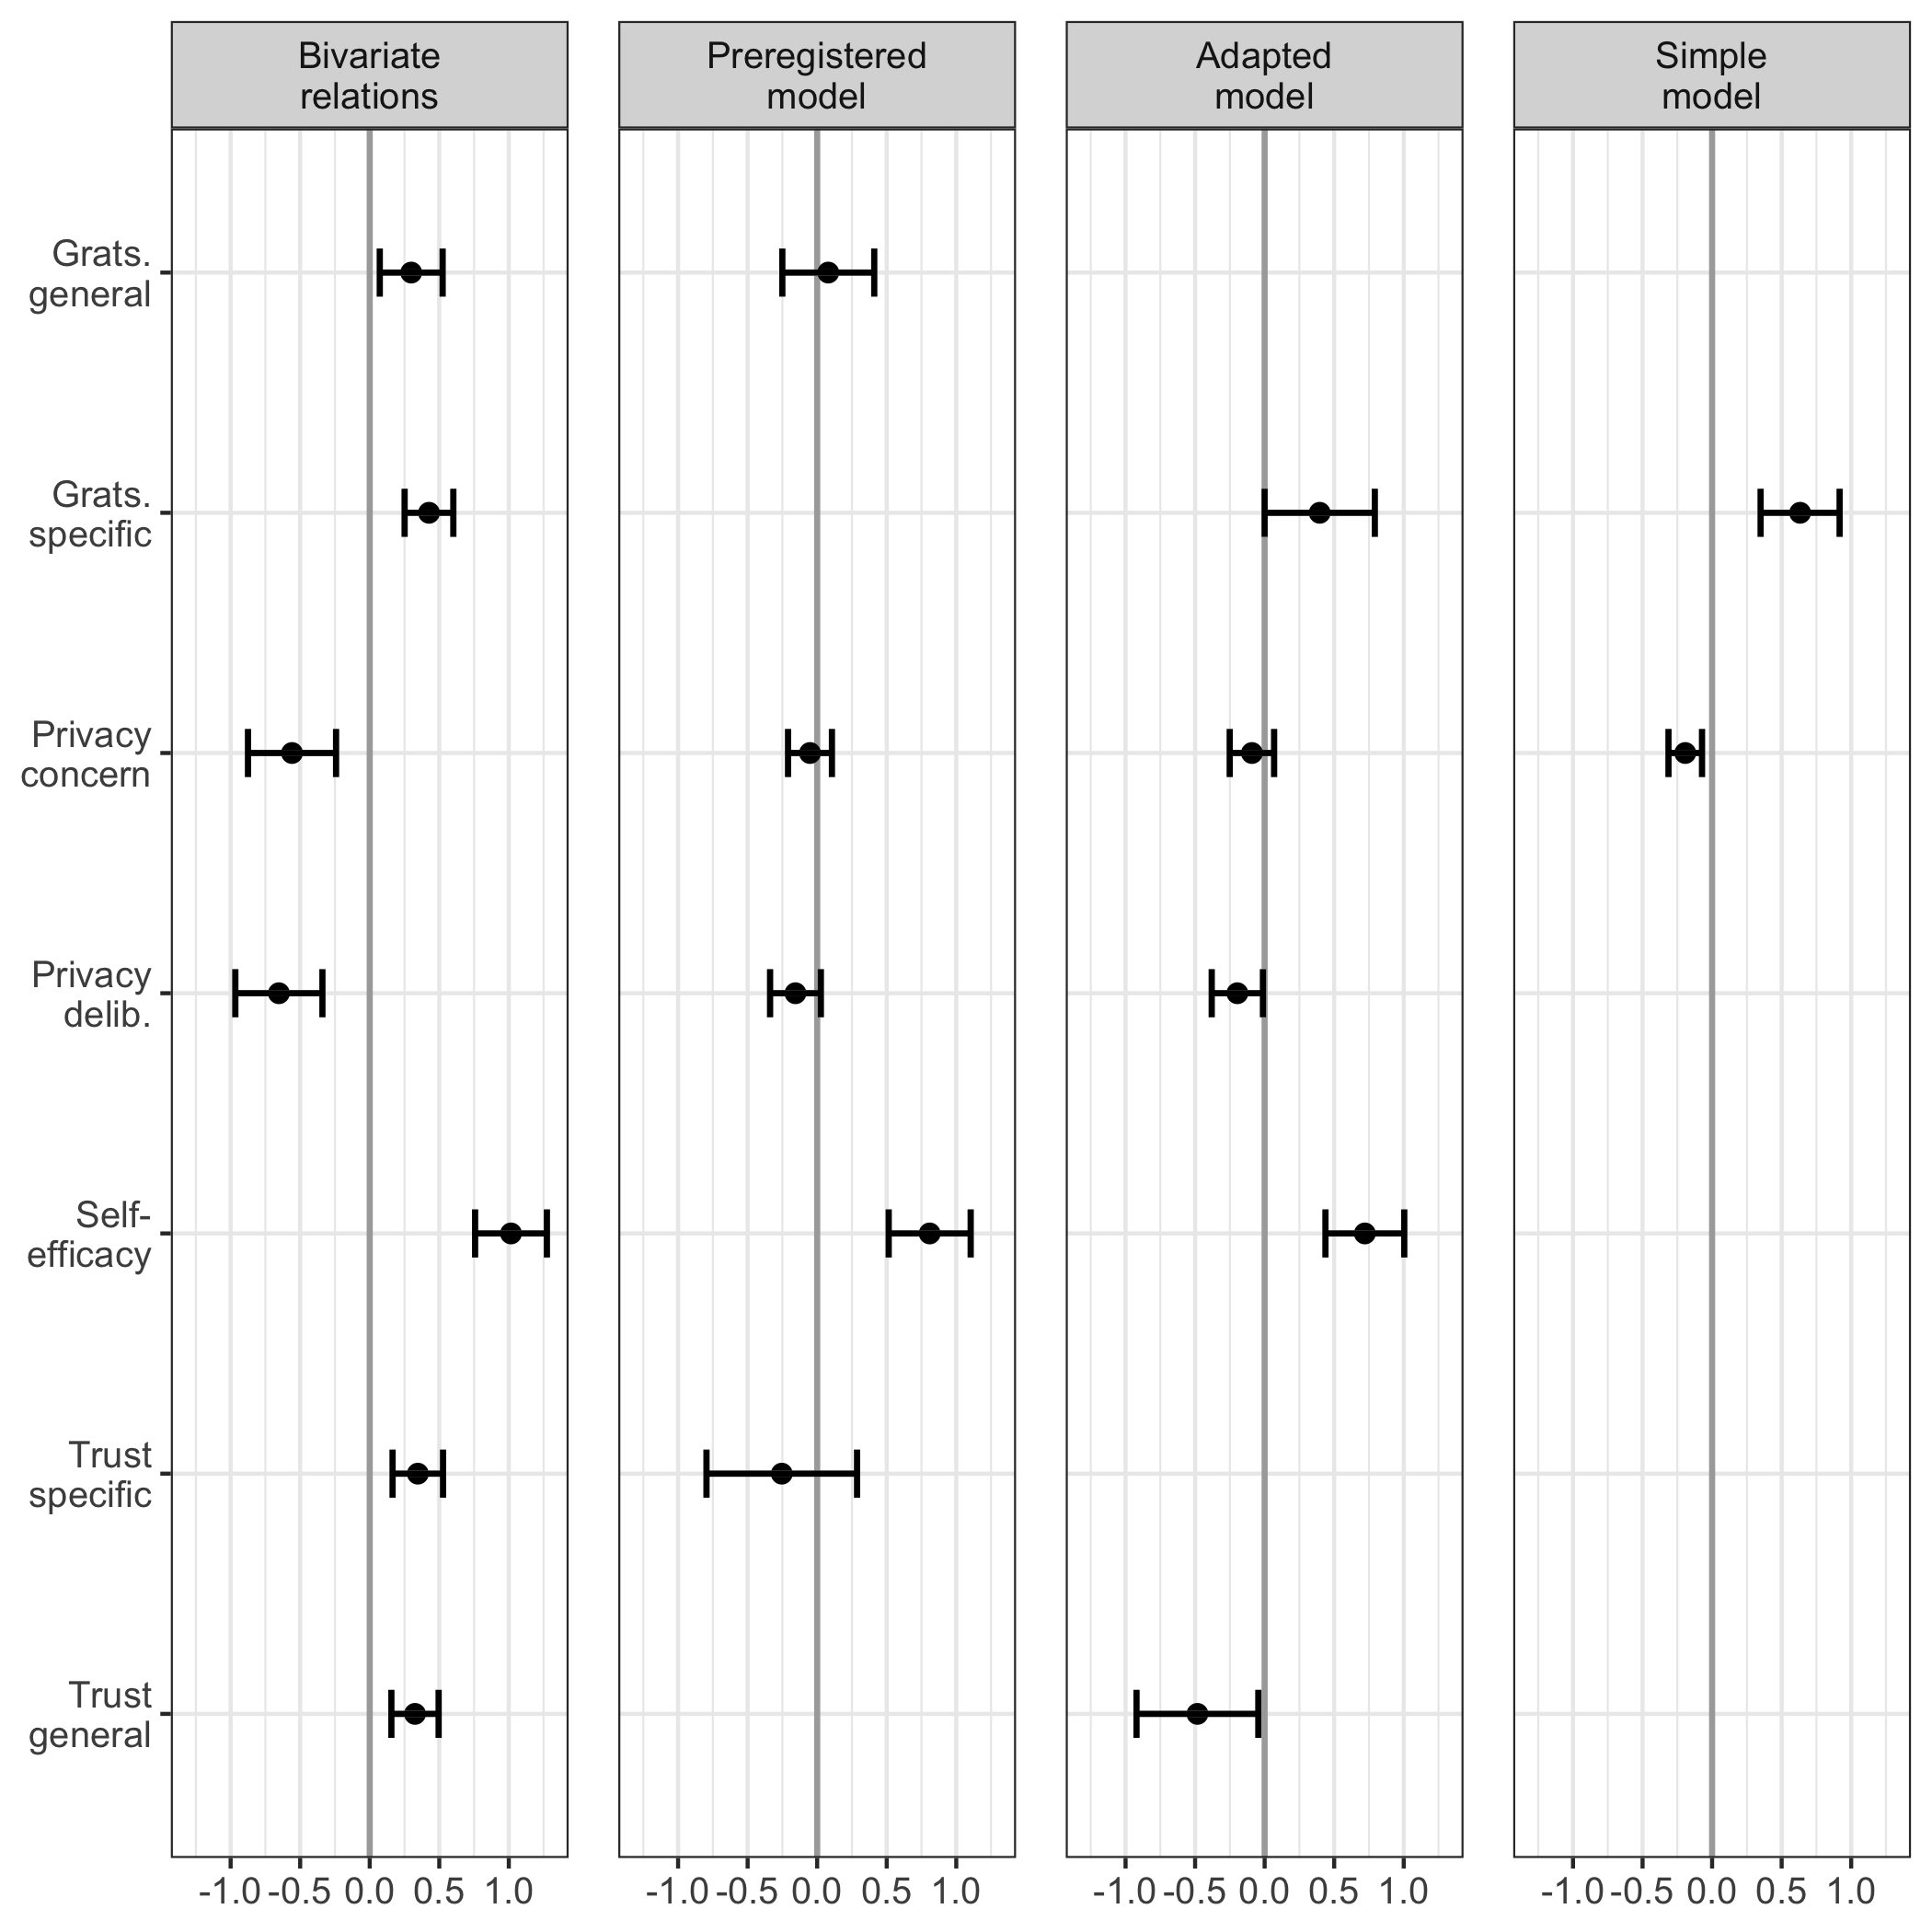
\includegraphics[width=\textwidth]{figures/results/coeffs} \caption{Predictors of self-disclosure. Displayed are the 95\% CIs of unstandardized effects.}\label{fig:plotpc}
\end{figure}

\hypertarget{popularity-cues}{%
\subsection{Popularity Cues}\label{popularity-cues}}

\hypertarget{preregistered-analyses-1}{%
\subsubsection{Preregistered analyses}\label{preregistered-analyses-1}}

In a next step, we analyzed the potential effects of the popularity cues.
We for example expected that websites with like buttons would lead to more self-disclosure, gratifications, and privacy deliberation and to less privacy concerns.
Somewhat surprisingly, we found no effects of the popularity cues on the privacy calculus variables.
For an illustration, see Figure \ref{fig:popularitycues}, which displays the model-predicted values for each variable (using the baseline model).
The results show that the confidence intervals of all preregistered variables overlap, illustrating that there were no statistically significant differences across websites.
For the detailed results of the specific inference tests using contrasts, see the OSM.

\hypertarget{exploratory-analyses-1}{%
\subsubsection{Exploratory analyses}\label{exploratory-analyses-1}}

The picture remained the same also when analyzing variables not included in the preregistration.
Note that some differences missed statistical significance only marginally (e.g., specific gratifications for the comparison between the website with like buttons and the control website without like and dislike buttons).
Nevertheless, we refrain from reading too much into these subtle differences.
We conclude that the three websites were comparable regarding the privacy calculus variables and the amount of self-disclosure.

\begin{figure}[!h]
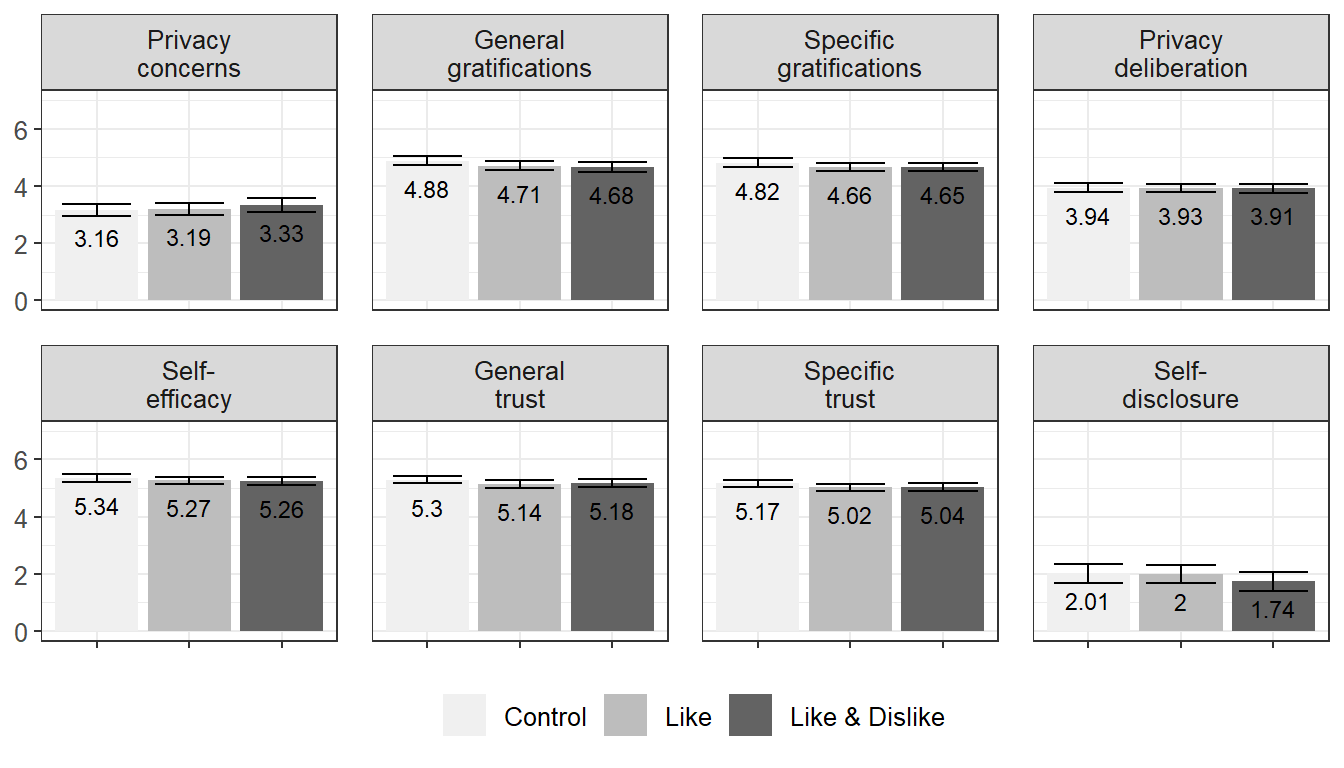
\includegraphics[width=\textwidth]{figures/results/bar_plot} \caption{Overview of the model-predicted values for each variable, separated for the three websites. Control: Website without buttons. Like: Website with like buttons. Like \& Dislike: Website with like and dislike buttons.}\label{fig:popularitycues}
\end{figure}

\hypertarget{discussion}{%
\section{Discussion}\label{discussion}}

This is the first study to analyze the privacy calculus using actual observed behavior in a preregistered field experiment.
The data stem from a representative sample of the German population.
We extended the theoretical privacy calculus model by explicitly testing privacy deliberation processes.
We included self-efficacy and trust as additional variables, to better represent our theoretical premise of bounded rationality.
We further asked whether the privacy calculus is affected by popularity cues such as like and dislike buttons.

In the bivariate analyses, all privacy calculus variables significantly predicted self-disclosure.
Thus, all variables likely play an important role when it comes to understanding online-processes.
In the preregistered analyses using multiple regression, however, only self-efficacy significantly predicted self-disclosure.
All other variables were not significant.
There seems to be a relevant overlap between variables, and their mutual relation is still not clear.
The preregistered extended privacy calculus model was therefore not supported by the data.
However, the model showed problems typical of multicollinearity, which is why we also explored (a) an adapted version of the preregistered model, in which we exchanged two variables, and (b) a simple privacy calculus model, which included only privacy concerns and specific gratifications.

The adapted model suggests that also when holding all other variables constant, people who deliberate more about their privacy disclose less.
People who expect more specific gratifications and who feel more self-efficacious disclose more.
However, the model also suggests that if trust increases, while all other factors remain constant, self-disclosure decreases, which seems theoretically implausible.
As a result, we also fit a simple privacy calculus model, which showed that both privacy concerns and obtained gratifications significantly and meaningfully predicted self-disclosure.
Taken together, the results support the privacy calculus framework and suggest that in specific contexts self-disclosure online is not erratic and that it can be explained by several psychological variables.
At the same time, variables such as trust and efficacy seem to play an important role, which further supports the underlying premise of bounded rationality.

The results suggest that in new communication contexts at least one third of all Internet users \emph{actively deliberates} about their privacy.
Determining whether this figure is large or small is difficult.
Although the effect seems substantial to us, one could argue that it should be higher and that more people should actively deliberate about their online self-disclosure.
Interestingly, results showed that privacy deliberation and privacy concerns were remarkably similar.
Both variables were strongly correlated and showed comparable correlations with other variables.
This either implies that thinking about privacy increases concerns or, conversely, that being concerned about privacy encourages us to ponder our options more carefully.
Future research might tell.

Popularity cues do not always seem to have a strong influence on the privacy calculus and self-disclosure.
Although some studies reported that popularity cues can substantially impact behavior (Muchnik, Aral, \& Taylor, 2013), in our study we found the opposite.
Users disclosed the same amount of personal information regardless of whether or not a website included like or dislike buttons.
The results do not imply that popularity cues have no impact on the privacy calculus in general.
Instead, they suggest that there exist certain contexts in which the influence of popularity cues is negligible.

The results also have methodological implications.
First, one can question the tendency to further increase the complexity of the privacy calculus model by adding additional variables (e.g., Dienlin \& Metzger, 2016).
``Since all models are wrong the scientist cannot obtain a''correct" one by excessive elaboration. {[}\ldots{]} Just as the ability to devise simple but evocative models is the signature of the great scientist so overelaboration and overparameterization is often the mark of mediocrity" (Box, 1976, p. 792).
For example, it seems that adding self-efficacy to privacy calculus models is of limited theoretical value.
Self-efficacy is often only a self-reported proxy of behavior and offers little incremental insight.
Instead, it might be more interesting to find out \emph{why} some people feel sufficiently efficacious to self-disclose whereas others do not.

In addition, although adding variables increases explained variance, it can also introduce multicollinearity.
Multicollinearity is not a problem per se, but rather a helpful warning sign (Vanhove, 2019).
From a \emph{statistical} perspective, strongly correlated predictors mean that standard errors become larger (Vanhove, 2019).
We can be less certain about the effects, because there is less unique variance (Vanhove, 2019).
As a remedy, researchers could collect larger samples, which would increase statistical power and precision.
Using accessible statistical software it is now possible to run a priori power analyses that explicitly account for correlated or collinear predictors (Wang \& Rhemtulla, 2020).

From a \emph{theoretical} perspective, multicollinearity could also suggest that the underlying theoretical model is ill-configured.
It is our understanding that multiple regression is often used to isolate effects, to make sure that they are not caused by other third variables.
However, in cases of highly correlated variables this often does not make much sense theoretically.
Combining trust and gratification in a multiple regression asks how increasing benefits affects self-disclosure \emph{while holding trust constant}.
However, it seems more plausible to assume that increasing gratifications also automatically increases trust (Söllner, Hoffmann, \& Leimeister, 2016).
In the preregistered analysis we even went further and tested whether trust increases self-disclose while holding constant gratifications, privacy concerns, privacy deliberations, and self-efficacy---an unlikely scenario.
In short, the effects we found could be correct, but the interpretation is more difficult, potentially artificial, and thereby of little theoretical and practical value.

Finally, we found a surprisingly strong correlation between specific trust and expected gratifications (i.e., \emph{r} = .79).
Operationalizations of trust are remarkably close to expected gratifications.
To illustrate, the trust subdimension \emph{ability} includes items such as ``The comments of other users were useful.''
Trust is often operationalized as a formative construct that directly results from factors such as expected benefits (Söllner, Hoffmann, \& Leimeister, 2016).
In conclusion, it is important not to confuse \emph{causes} of trust with \emph{measures} of trust.
We thus recommend using general and reflective measures of trust.

\hypertarget{limitations}{%
\subsection{Limitations}\label{limitations}}

This paper operationalized self-disclosure via communication quantity.
Other understandings of self-disclosure exist that are more narrow, and that would require a qualitative analysis of exchanged communication.
However, additional qualitative analyses were beyond the scope of this paper and not aligned with our theoretical understanding of self-disclosure.

Although we did not find significant effects of like and dislike buttons in this study, they could still affect the privacy calculus in other contexts and settings.
Our findings are limited to the context we analyzed and should not be overly generalized.
Null-findings pose the \emph{Duhème-Quinn Problem} (Dienes, 2008).
They can either result from an actual non-existence of effects or, instead, from a poor operationalization of the research question.
In this case, we were not able send participants notifications when their comments were liked or disliked, which significantly decreased the popularity cues' salience.

The results do not allow for causal interpretation.
First, all results are based on analyses of between-person variance.
However, between-person relations often do not translate to within-person effects (Hamaker, Kuiper, \& Grasman, 2015).
Likewise, the mediation model is only suggestive, as we did not experimentally manipulate the mediating variables and also did not use a longitudinal design.

The self-reported measures were collected \emph{after} the field phase in which the dependent variable was measured.
As a result, the coefficients might overestimate the actual relations, because demand effects might have led participants to artificially align their theoretical answers with their practical behavior.

The assumption of stable unit treatment states that in experiments only the experimental variable should be manipulated, while all others should be held constant (Kline, 2016).
In this study, we explicitly manipulated the popularity cues.
However, because the experiment was conducted in the field several other variables could not be held constant, such as the content of communication by other users, the unfolding communication dynamics, and the characteristics of other users.
As a result, the assumption of stable unit treatment was violated.

\hypertarget{conclusion}{%
\subsection{Conclusion}\label{conclusion}}

In this study we have found some support for the privacy calculus approach.
People who were more concerned about their privacy disclosed less information online, whereas people who received more gratifications from using a website disclosed more information online.
A substantial share of internet users, approximately 30\%, engaged in a privacy calculus by actively deliberating about whether or not to disclose information.
Popularity cues such as like and dislike buttons played only a minor role in this process.
In conclusion, the results provide further evidence against the privacy paradox.
Internet users are at least somewhat proactive and reasonable---maybe no more or less proactive or reasonable than in other everyday situations.

\newpage

\hypertarget{references}{%
\section{References}\label{references}}

\setlength{\parindent}{-0.5in}
\setlength{\leftskip}{0.5in}

\hypertarget{refs}{}
\begin{CSLReferences}{1}{0}
\leavevmode\hypertarget{ref-altmanPrivacyConceptualAnalysis1976}{}%
Altman, I. (1976). Privacy: {A} conceptual analysis. \emph{Environment and Behavior}, \emph{8}(1), 7--29. \url{https://doi.org/10.1177/001391657600800102}

\leavevmode\hypertarget{ref-R-papaja}{}%
Aust, F., \& Barth, M. (2018). \emph{{papaja}: {Create} {APA} manuscripts with {R Markdown}}. Retrieved from \url{https://github.com/crsh/papaja}

\leavevmode\hypertarget{ref-barnesPrivacyParadoxSocial2006}{}%
Barnes, S. B. (2006). A privacy paradox: {Social} networking in the {United} {States}. \emph{First Monday}, \emph{11}(9). Retrieved from \href{https://www.firstmonday.org/issues/issue11_9/barnes/index.html}{www.firstmonday.org/issues/issue11\_9/barnes/index.html}

\leavevmode\hypertarget{ref-baruhOnlinePrivacyConcerns2017}{}%
Baruh, L., Secinti, E., \& Cemalcilar, Z. (2017). Online privacy concerns and privacy management: {A} meta-analytical review. \emph{Journal of Communication}, \emph{67}(1), 26--53. \url{https://doi.org/10.1111/jcom.12276}

\leavevmode\hypertarget{ref-R-quanteda}{}%
Benoit, K. (2018). \emph{Quanteda: Quantitative analysis of textual data}. \url{https://doi.org/10.5281/zenodo.1004683}

\leavevmode\hypertarget{ref-bolUnderstandingEffectsPersonalization2018}{}%
Bol, N., Dienlin, T., Kruikemeier, S., Sax, M., Boerman, S. C., Strycharz, J., \ldots{} Vreese, C. H. (2018). Understanding the effects of personalization as a privacy calculus: {Analyzing} self-disclosure across health, news, and commerce contexts. \emph{Journal of Computer-Mediated Communication}, \emph{23}(6), 370--388. \url{https://doi.org/10.1093/jcmc/zmy020}

\leavevmode\hypertarget{ref-boxScienceStatistics1976}{}%
Box, G. E. P. (1976). Science and statistics. \emph{Journal of the American Statistical Association}, \emph{71}(356), 791--799. \url{https://doi.org/10.1080/01621459.1976.10480949}

\leavevmode\hypertarget{ref-buchananDevelopmentMeasuresOnline2007}{}%
Buchanan, T., Paine, C., Joinson, A. N., \& Reips, U.-D. (2007). Development of measures of online privacy concern and protection for use on the {Internet}. \emph{Journal of the American Society for Information Science and Technology}, \emph{58}(2), 157--165. \url{https://doi.org/10.1002/asi.20459}

\leavevmode\hypertarget{ref-carrPredictingThresholdPerceived2018}{}%
Carr, C. T., Hayes, R. A., \& Sumner, E. M. (2018). Predicting a threshold of perceived {Facebook} post success via likes and reactions: {A} test of explanatory mechanisms. \emph{Communication Research Reports}, \emph{35}(2), 141--151. \url{https://doi.org/10.1080/08824096.2017.1409618}

\leavevmode\hypertarget{ref-R-pwr}{}%
Champely, S. (2018). \emph{Pwr: Basic functions for power analysis}. Retrieved from \url{https://CRAN.R-project.org/package=pwr}

\leavevmode\hypertarget{ref-chenRevisitingPrivacyParadox2018}{}%
Chen, H.-T. (2018). Revisiting the privacy paradox on social media with an extended privacy calculus model: {The} effect of privacy concerns, privacy self-efficacy, and social capital on privacy management. \emph{American Behavioral Scientist}, \emph{62}(10), 1392--1412. \url{https://doi.org/10.1177/0002764218792691}

\leavevmode\hypertarget{ref-cohenPowerPrimer1992}{}%
Cohen, J. (1992). A power primer. \emph{Psychological Bulletin}, \emph{112}(1), 155--159. \url{https://doi.org/10.1037/0033-2909.112.1.155}

\leavevmode\hypertarget{ref-dhirUnderstandingRelationshipIntensity2017}{}%
Dhir, A., \& Tsai, C.-C. (2017). Understanding the relationship between intensity and gratifications of {Facebook} use among adolescents and young adults. \emph{Telematics and Informatics}, \emph{34}(4), 350--364. \url{https://doi.org/10.1016/j.tele.2016.08.017}

\leavevmode\hypertarget{ref-dienesUnderstandingPsychologyScience2008}{}%
Dienes, Z. (2008). \emph{Understanding psychology as a science: {An} introduction to scientific and statistical inference}. New York, N.Y.: Palgrave Macmillan.

\leavevmode\hypertarget{ref-dienlinPsychologyPrivacyAnalyzing2017}{}%
Dienlin, T. (2017). \emph{The psychology of privacy: {Analyzing} processes of media use and interpersonal communication}. Hohenheim, Germany: University of Hohenheim. Retrieved from \url{http://opus.uni-hohenheim.de/volltexte/2017/1315/}

\leavevmode\hypertarget{ref-dienlinLongitudinalAnalysisPrivacy2019}{}%
Dienlin, T., Masur, P. K., \& Trepte, S. (2019). \emph{A longitudinal analysis of the privacy paradox} (preprint). SocArXiv. \url{https://doi.org/10.31235/osf.io/fm4h7}

\leavevmode\hypertarget{ref-dienlinExtendedPrivacyCalculus2016}{}%
Dienlin, T., \& Metzger, M. J. (2016). An extended privacy calculus model for {SNSs}: {Analyzing} self-disclosure and self-withdrawal in a representative {U}.{S}. sample. \emph{Journal of Computer-Mediated Communication}, \emph{21}(5), 368--383. \url{https://doi.org/10.1111/jcc4.12163}

\leavevmode\hypertarget{ref-ellisonSocialNetworkSite2015}{}%
Ellison, N. B., \& Vitak, J. (2015). Social network site affordances and their relationship to social capital processes. In S. S. Sundar (Ed.), \emph{The handbook of the psychology of communication technology} (Vol. v.33, pp. 205--227). Chichester, MA: Wiley Blackwell.

\leavevmode\hypertarget{ref-ellisonNegotiatingPrivacyConcerns2011}{}%
Ellison, N. B., Vitak, J., Steinfield, C., Gray, R., \& Lampe, C. (2011). Negotiating privacy concerns and social capital needs in a social media environment. In S. Trepte \& L. Reinecke (Eds.), \emph{Privacy online: {Perspectives} on privacy and self-disclosure in the social web} (pp. 19--32). Berlin, Germany: Springer. \url{https://doi.org/10.1007/978-3-642-21521-6_3}

\leavevmode\hypertarget{ref-foxDistinguishingTechnologiesSocial2017}{}%
Fox, J., \& McEwan, B. (2017). Distinguishing technologies for social interaction: {The} perceived social affordances of communication channels scale. \emph{Communication Monographs}, \emph{9}, 1--21. \url{https://doi.org/10.1080/03637751.2017.1332418}

\leavevmode\hypertarget{ref-gefenTrustTAMOnline2003}{}%
Gefen, D., Karahanna, E., \& Straub, D. W. (2003). Trust and {TAM} in online shopping: {An} integrated model. \emph{MIS Q}, \emph{27}(1), 5190. Retrieved from \url{http://dl.acm.org/citation.cfm?id=2017181.2017185}

\leavevmode\hypertarget{ref-gibsonEcologicalApproachVisual2015}{}%
Gibson, J. J. (2015). \emph{The ecological approach to visual perception}. New York, NY: Psychology Press.

\leavevmode\hypertarget{ref-grewalMulticollinearityMeasurementError2004}{}%
Grewal, R., Cote, J. A., \& Baumgartner, H. (2004). Multicollinearity and measurement error in structural equation models: {Implications} for theory testing. \emph{Marketing Science}, \emph{23}(4), 519--529. \url{https://doi.org/10.1287/mksc.1040.0070}

\leavevmode\hypertarget{ref-hamakerCritiqueCrosslaggedPanel2015}{}%
Hamaker, E. L., Kuiper, R. M., \& Grasman, R. P. P. P. (2015). A critique of the cross-lagged panel model. \emph{Psychological Methods}, \emph{20}(1), 102--116. \url{https://doi.org/10.1037/a0038889}

\leavevmode\hypertarget{ref-heirmanPredictingAdolescentsDisclosure2013}{}%
Heirman, W., Walrave, M., \& Ponnet, K. (2013). Predicting adolescents' disclosure of personal information in exchange for commercial incentives: {An} application of an extended theory of planned behavior. \emph{Cyberpsychology, Behavior, and Social Networking}, \emph{16}(2), 81--87. \url{https://doi.org/10.1089/cyber.2012.0041}

\leavevmode\hypertarget{ref-R-semTools}{}%
Jorgensen, D., T., Pornprasertmanit, S., Schoemann, M., A., \ldots{} Y. (2018). \emph{{semTools}: Useful tools for structural equation modeling}. Retrieved from \url{https://CRAN.R-project.org/package=semTools}

\leavevmode\hypertarget{ref-jourardTransparentSelf1964}{}%
Jourard, S. M. (1964). \emph{The transparent self}. New York, NY: Van Nostrand.

\leavevmode\hypertarget{ref-kahnemanThinkingFastSlow2011}{}%
Kahneman, D. (2011). \emph{Thinking, fast and slow}. New York: Farrar, Straus; Giroux.

\leavevmode\hypertarget{ref-klinePrinciplesPracticeStructural2016}{}%
Kline, R. B. (2016). \emph{Principles and practice of structural equation modeling} (4th ed.). New York, NY: The Guilford Press.

\leavevmode\hypertarget{ref-knijnenburgDeathPrivacyCalculus2017}{}%
Knijnenburg, B., Raybourn, E., Cherry, D., Wilkinson, D., Sivakumar, S., \& Sloan, H. (2017). Death to the privacy calculus? \emph{SSRN Electronic Journal}. \url{https://doi.org/10.2139/ssrn.2923806}

\leavevmode\hypertarget{ref-kokolakisPrivacyAttitudesPrivacy2017}{}%
Kokolakis, S. (2017). Privacy attitudes and privacy behaviour: {A} review of current research on the privacy paradox phenomenon. \emph{Computers \& Security}, \emph{64}, 122--134. \url{https://doi.org/10.1016/j.cose.2015.07.002}

\leavevmode\hypertarget{ref-koohikamaliInvestigationDynamicModel2019}{}%
Koohikamali, M., French, A. M., \& Kim, D. J. (2019). An investigation of a dynamic model of privacy trade-off in use of mobile social network applications: {A} longitudinal perspective. \emph{Decision Support Systems}, \emph{119}, 46--59. \url{https://doi.org/10.1016/j.dss.2019.02.007}

\leavevmode\hypertarget{ref-kosinskiPrivateTraitsAttributes2013}{}%
Kosinski, M., Stillwell, D., \& Graepel, T. (2013). Private traits and attributes are predictable from digital records of human behavior. \emph{Proceedings of the National Academy of Sciences of the United States of America}, \emph{110}(15), 5802--5805. \url{https://doi.org/10.1073/pnas.1218772110}

\leavevmode\hypertarget{ref-krasnovaOnlineSocialNetworks2010}{}%
Krasnova, H., Spiekermann, S., Koroleva, K., \& Hildebrand, T. (2010). Online social networks: {Why} we disclose. \emph{Journal of Information Technology}, \emph{25}(2), 109--125. \url{https://doi.org/10.1057/jit.2010.6}

\leavevmode\hypertarget{ref-kramerMasteringChallengeBalancing2020}{}%
Krämer, N. C., \& Schäwel, J. (2020). Mastering the challenge of balancing self-disclosure and privacy in social media. \emph{Current Opinion in Psychology}, \emph{31}, 67--71. \url{https://doi.org/10.1016/j.copsyc.2019.08.003}

\leavevmode\hypertarget{ref-lakensEquivalenceTestingPsychological2018}{}%
Lakens, D., Scheel, A. M., \& Isager, P. M. (2018). Equivalence testing for psychological research: {A} tutorial. \emph{Advances in Methods and Practices in Psychological Science}, \emph{1}(2), 259--269. \url{https://doi.org/10.1177/2515245918770963}

\leavevmode\hypertarget{ref-lauferPrivacyConceptSocial1977}{}%
Laufer, R. S., \& Wolfe, M. (1977). Privacy as a concept and a social issue: {A} multidimensional developmental theory. \emph{Journal of Social Issues}, \emph{33}(3), 22--42. \url{https://doi.org/10.1111/j.1540-4560.1977.tb01880.x}

\leavevmode\hypertarget{ref-liEmpiricalStudiesOnline2011}{}%
Li, Y. (2011). Empirical studies on online information privacy concerns: {Literature} review and an integrative framework. \emph{Communications of the Association for Information Systems}, \emph{28}, 453--496.

\leavevmode\hypertarget{ref-masurSituationalPrivacySelfdisclosure2018}{}%
Masur, P. K. (2018). \emph{Situational privacy and self-disclosure: {Communication} processes in online environments}. Cham, Switzerland: Springer.

\leavevmode\hypertarget{ref-metzgerPrivacyTrustDisclosure2004}{}%
Metzger, M. J. (2004). Privacy, trust, and disclosure: {Exploring} barriers to electronic commerce. \emph{Journal of Computer-Mediated Communication}, \emph{9}(4). \url{https://doi.org/10.1111/j.1083-6101.2004.tb00292.x}

\leavevmode\hypertarget{ref-minHowArePeople2015}{}%
Min, J., \& Kim, B. (2015). How are people enticed to disclose personal information despite privacy concerns in social network sites? {The} calculus between benefit and cost. \emph{Journal of the Association for Information Science and Technology}, \emph{66}(4), 839--857. \url{https://doi.org/10.1002/asi.23206}

\leavevmode\hypertarget{ref-muchnikSocialInfluenceBias2013}{}%
Muchnik, L., Aral, S., \& Taylor, S. J. (2013). Social influence bias: {A} randomized experiment. \emph{Science (New York, N.Y.)}, \emph{341}(6146), 647--651. \url{https://doi.org/10.1126/science.1240466}

\leavevmode\hypertarget{ref-newyorkpublicradioPrivacyParadox2018}{}%
New York Public Radio. (2018). The privacy paradox. \{InternetDocument\}. Retrieved from \url{https://project.wnyc.org/privacy-paradox/}

\leavevmode\hypertarget{ref-omarzuDisclosureDecisionModel2000}{}%
Omarzu, J. (2000). A disclosure decision model: {Determining} how and when individuals will self-disclose. \emph{Personality and Social Psychology Review}, \emph{4}(2), 174--185. \url{https://doi.org/10.1207/S15327957PSPR0402_5}

\leavevmode\hypertarget{ref-pettyCommunicationPersuasionCentral1986}{}%
Petty, R., \& Cacioppo, J. (1986). \emph{Communication and {Persuasion}: {Central} and {Peripheral} {Routes} to {Attitude} {Change}}. New York: Springer-Verlag. \url{https://doi.org/10.1007/978-1-4612-4964-1}

\leavevmode\hypertarget{ref-R-base}{}%
R Core Team. (2018). \emph{R: A language and environment for statistical computing}. Vienna, Austria: R Foundation for Statistical Computing. Retrieved from \url{https://www.R-project.org/}

\leavevmode\hypertarget{ref-reineckeAuthenticityWellbeingSocial2014}{}%
Reinecke, L., \& Trepte, S. (2014). Authenticity and well-being on social network sites: {A} two-wave longitudinal study on the effects of online authenticity and the positivity bias in {SNS} communication. \emph{Computers in Human Behavior}, \emph{30}, 95--102. \url{https://doi.org/10.1016/j.chb.2013.07.030}

\leavevmode\hypertarget{ref-rosoffHeuristicsBiasesCyber2013}{}%
Rosoff, H., Cui, J., \& John, R. S. (2013). Heuristics and biases in cyber security dilemmas. \emph{Environment Systems and Decisions}, \emph{33}(4), 517--529. \url{https://doi.org/10.1007/s10669-013-9473-2}

\leavevmode\hypertarget{ref-R-lavaan}{}%
Rosseel, Y. (2012). {lavaan}: An {R} package for structural equation modeling. \emph{Journal of Statistical Software}, \emph{48}(2), 1--36. Retrieved from \url{http://www.jstatsoft.org/v48/i02/}

\leavevmode\hypertarget{ref-schererGratifikationMinuteZeitnahe2002}{}%
Scherer, H., \& Schlütz, D. (2002). Gratifikation à la minute: {Die} zeitnahe {Erfassung} von {Gratifikationen}. In P. Rössler (Ed.), \emph{Empirische {Perspektiven} der {Rezeptionsforschung}} (pp. 133--151). Munich, Germany: Reinhard Fischer.

\leavevmode\hypertarget{ref-simonBoundedRationality1990}{}%
Simon, H. A. (1990). Bounded {Rationality}. In J. Eatwell, M. Milgate, \& P. Newman (Eds.), \emph{Utility and {Probability}} (pp. 15--18). London: Palgrave Macmillan UK. \url{https://doi.org/10.1007/978-1-349-20568-4_5}

\leavevmode\hypertarget{ref-sollnerWhyDifferentTrust2016}{}%
Söllner, M., Hoffmann, A., \& Leimeister, J. M. (2016). Why different trust relationships matter for information systems users. \emph{European Journal of Information Systems}, \emph{25}(3), 274--287. \url{https://doi.org/10.1057/ejis.2015.17}

\leavevmode\hypertarget{ref-stroudRecommendRespectAltering2017}{}%
Stroud, N. J., Muddiman, A., \& Scacco, J. M. (2017). Like, recommend, or respect?: {Altering} political behavior in news comment sections. \emph{New Media \& Society}, \emph{19}(11), 1727--1743. \url{https://doi.org/10.1177/1461444816642420}

\leavevmode\hypertarget{ref-sumnerFunctionalApproachFacebook2017}{}%
Sumner, E. M., Ruge-Jones, L., \& Alcorn, D. (2017). A functional approach to the {Facebook} {Like} button: {An} exploration of meaning, interpersonal functionality, and potential alternative response buttons. \emph{New Media \& Society}, \emph{20}(4), 1451--1469. \url{https://doi.org/10.1177/1461444817697917}

\leavevmode\hypertarget{ref-sunLocationInformationDisclosure2015}{}%
Sun, Y., Wang, N., Shen, X.-L., \& Zhang, J. X. (2015). Location information disclosure in location-based social network services: {Privacy} calculus, benefit structure, and gender differences. \emph{Computers in Human Behavior}, \emph{52}, 278--292. \url{https://doi.org/10.1016/j.chb.2015.06.006}

\leavevmode\hypertarget{ref-taddickenUsesPrivacyOnline2011}{}%
Taddicken, M., \& Jers, C. (2011). The uses of privacy online: {Trading} a loss of privacy for social web gratifications? In S. Trepte \& L. Reinecke (Eds.), \emph{Privacy online: {Perspectives} on privacy and self-disclosure in the social web} (pp. 143--158). Berlin, Germany: Springer.

\leavevmode\hypertarget{ref-tifferetGenderDifferencesPrivacy2019}{}%
Tifferet, S. (2019). Gender differences in privacy tendencies on social network sites: {A} meta-analysis. \emph{Computers in Human Behavior}, \emph{93}, 1--12. \url{https://doi.org/10.1016/j.chb.2018.11.046}

\leavevmode\hypertarget{ref-treptePrivacyCalculusContextualized2020}{}%
Trepte, S., Scharkow, M., \& Dienlin, T. (2020). The privacy calculus contextualized: {The} influence of affordances. \emph{Computers in Human Behavior}, \emph{104}, 106115. \url{https://doi.org/10.1016/j.chb.2019.08.022}

\leavevmode\hypertarget{ref-vanhoveCollinearityIsnDisease2019}{}%
Vanhove, J. (2019). Collinearity isn't a disease that needs curing. Retrieved from \url{https://osf.io/8x4uc/}

\leavevmode\hypertarget{ref-wangPowerAnalysisParameter2020}{}%
Wang, Y. A., \& Rhemtulla, M. (2020). Power analysis for parameter estimation in structural equation modeling: {A} discussion and tutorial. \url{https://doi.org/10.31234/osf.io/pj67b}

\leavevmode\hypertarget{ref-watzlawickPragmaticsHumanCommunication2011}{}%
Watzlawick, P., Bavelas, J. B., Jackson, D. D., \& O'Hanlon, B. (2011). \emph{Pragmatics of human communication: {A} study of interactional patterns, pathologies, and paradoxes}. New York, NY: W.W. Norton \& Co.

\leavevmode\hypertarget{ref-whitingWhyPeopleUse2013}{}%
Whiting, A., \& Williams, D. (2013). Why people use social media: A uses and gratifications approach. \emph{Qualitative Market Research: An International Journal}, \emph{16}(4), 362--369. \url{https://doi.org/10.1108/QMR-06-2013-0041}

\leavevmode\hypertarget{ref-R-tidyverse}{}%
Wickham, H. (2017). \emph{Tidyverse: Easily install and load the 'tidyverse'}. Retrieved from \url{https://CRAN.R-project.org/package=tidyverse}

\end{CSLReferences}


\end{document}
